%%%%%%%%%%%%%%%%%%%%%%%%%%%%%%%%%%%%%%%%%%  不使用 authblk 包制作标题  %%%%%%%%%%%%%%%%%%%%%%%%%%%%%%%%%%%%%%%%%%%%%%
%-------------------------------PPT Title-------------------------------------
\title{23-选讲专题:~机器学习算法简介}
%-----------------------------------------------------------------------------
%----------------------------Author & Date------------------------------------

%\author[\textrm{Jun\_Jiang}]{姜\;\;骏\inst{}} %[]{} (optional, use only with lots of authors)
%% - Give the names in the same order as the appear in the paper.
%% - Use the \inst{?} command only if the authors have different
%%   affiliation.
%\institute[BCC]{\inst{}%
\institute[Gain~Strong]{\inst{}%
%\vskip -20pt 北京市计算中心}
\vskip -20pt {\large 格致斯创~科技}}
\date[\today] % (optional, should be abbreviation of conference name)
{%	{\fontsize{6.2pt}{4.2pt}\selectfont{\textcolor{blue}{E-mail:~}\url{jiangjun@bcc.ac.cn}}}
\vskip 45 pt {\fontsize{8.2pt}{6.2pt}\selectfont{%清华大学\;\;物理系% 报告地点
	\vskip 5 pt \textrm{2023.11.18}}}
}

%% - Either use conference name or its abbreviation
%% - Not really information to the audience, more for people (including
%%   yourself) who are reading the slides onlin%%   yourself) who are reading the slides onlin%%   yourself) who are reading the slides onlineee
%%%%%%%%%%%%%%%%%%%%%%%%%%%%%%%%%%%%%%%%%%%%%%%%%%%%%%%%%%%%%%%%%%%%%%%%%%%%%%%%%%%%%%%%%%%%%%%%%%%%%%%%%%%%%%%%%%%%%

\subject{}
% This is only inserted into the PDF information catalog. Can be left
% out.
%\maketitle
\frame
{
%	\frametitle{\fontsize{9.5pt}{5.2pt}\selectfont{\textcolor{orange}{“高通量并发式材料计算算法与软件”年度检查}}}
\titlepage
}
%-----------------------------------------------------------------------------

%------------------------------------------------------------------------------列出全文 outline ---------------------------------------------------------------------------------
%\section*{}
%\frame[allowframebreaks]
%{
%  \frametitle{Outline}
%%  \frametitle{\textcolor{mycolor}{\secname}}
%  \tableofcontents%[current,currentsection,currentsubsection]
%}
%%在每个section之前列出全部Outline
%%类似的在每个subsection之前列出全部Outline是\AtBeginSubsection[]
%\AtBeginSection[]
%{
%  \frame<handout:0>%[allowframebreaks]
%  {
%    \frametitle{Outline}
%%全部Outline中,本部分加亮
%    \tableofcontents[current,currentsection]
%  }
%}

%-----------------------------------------------PPT main Body------------------------------------------------------------------------------------
\small
%\section{\rm{VASP~}软件中\rm{PAW~}计算的实现}
%\frame
%
%	\frametitle{\textrm{VASP}计算的特色}
%	相比于与普通的第一原理计算软件,\textrm{VASP}很好地平衡了计算效率和精度的问题,总的来说,\textrm{VASP}主要通过这几个特色保证了计算的高效能
%	\begin{itemize}
%	     \item 迭代与优化算法的多样性\\
%		     本质上电荷密度迭代 \textrm{\&\&} 体系总能量优化是相同的优化问题,采用了类似的算法\upcite{CMS6-15_1996,PRB54-11169_1996}:\\
%			\textcolor{blue}{\textrm{Pseudo-Newton、Conjugate-Gradient、Broyden~mix、damping-factor、RMM-DIIS}}
%	     \item 尽可能采用局域基(原子轨道基)函数:~\\
%		     \textcolor{blue}{\textrm{LREAL}}=\textcolor{red}{\textrm{.TRUE.}}\\
%			优化的投影函数也尽可能在实空间表示
%	     \item \textrm{PAW}原子数据集:\textcolor{blue}{优异的赝势}\upcite{PRB59-1758_1999}
%	\end{itemize}
%}
\frame
{
	\frametitle{科学研究的范式变更}
\begin{figure}[h!]
\vspace*{0.08in}
\centering
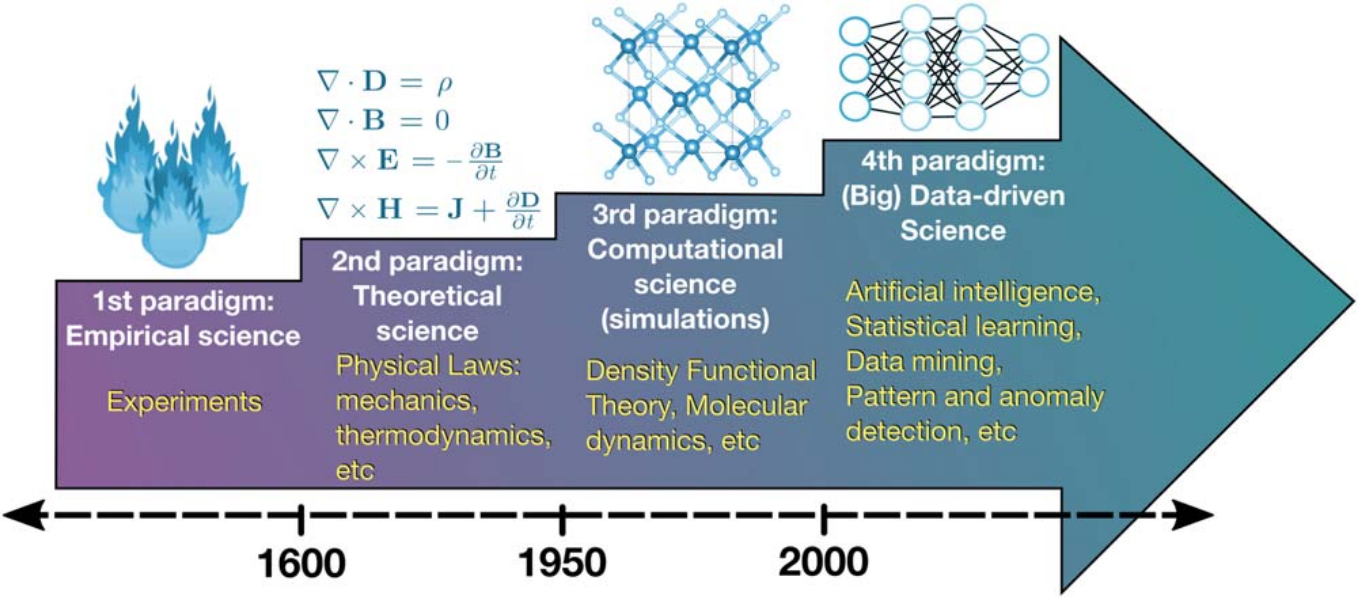
\includegraphics[height=2.00in,width=4.15in]{Figures/Four_Model_3.png}
%\caption{\tiny \textrm{Pseudopotential for metallic sodium, based on the empty core model and screened by the Thomas-Fermi dielectric function.}}%(与文献\cite{EPJB33-47_2003}图1对比)
\label{Four_Model}
\end{figure}
}

\frame
{
	\frametitle{数据驱动的科学研究}
前所未有的计算能力和大规模的数据收集能力%,现代科学正在进入“第四范式”:
\begin{figure}[h!]
%\vspace*{-0.05in}
\centering
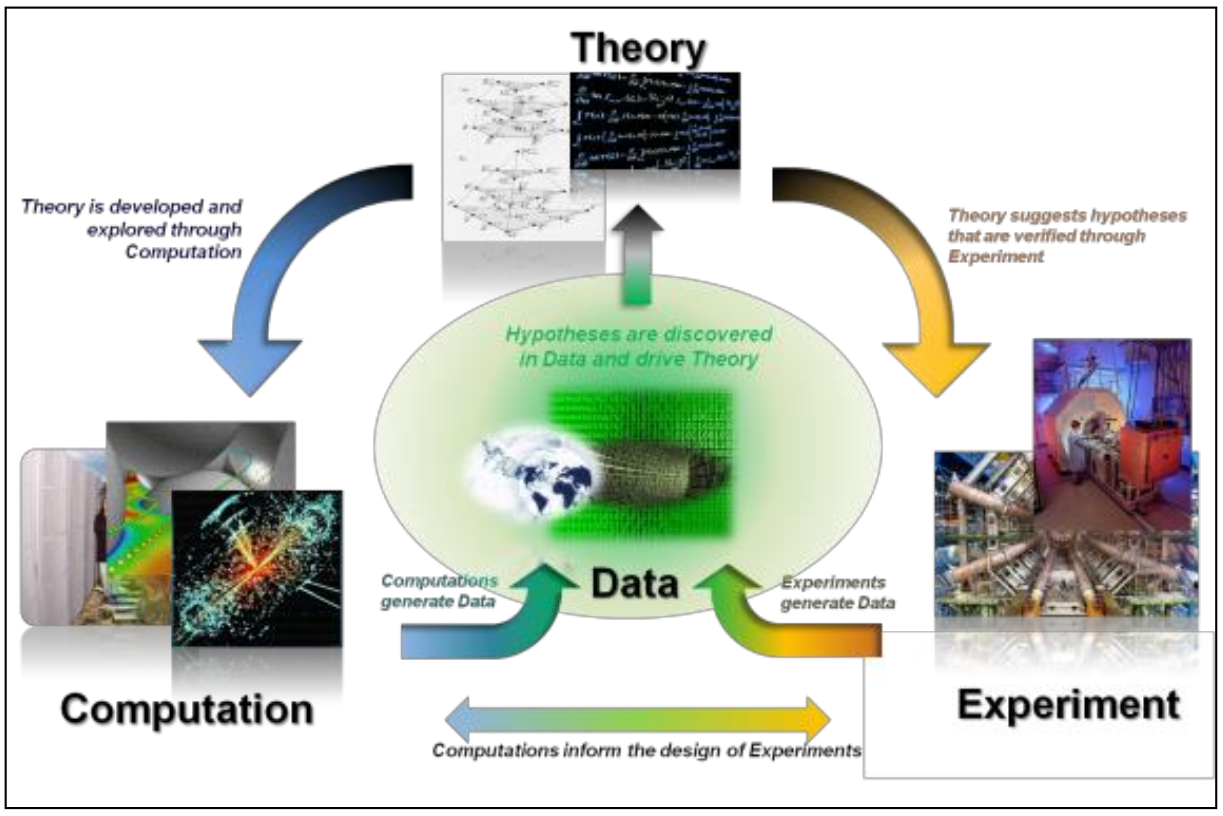
\includegraphics[height=2.40in,width=3.75in]{Figures/Four_Model_1.png}
%\caption{\tiny \textrm{Pseudopotential for metallic sodium, based on the empty core model and screened by the Thomas-Fermi dielectric function.}}%(与文献\cite{EPJB33-47_2003}图1对比)
\label{Four_Model_1}
\end{figure}
科学的新驱动力:~\textcolor{red}{密集数据}+\textcolor{red}{人工智能}
}

\section{机器学习简介}
\frame
{
	\frametitle{机器学习\textrm{(Machine Learning, ML)}}
机器学习是自动完成数据分析并提取数据关系的一类方法的统称
\begin{figure}[h!]
\centering
\vspace*{-0.1in}
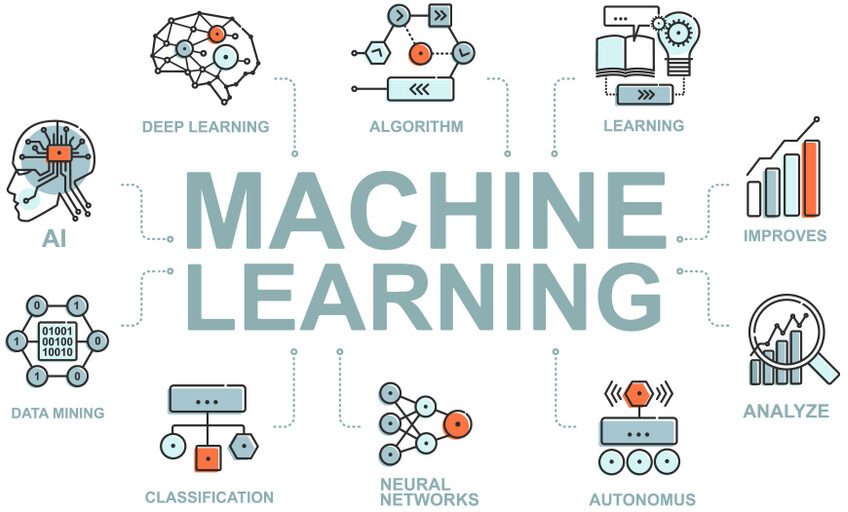
\includegraphics[height=2.3in,width=3.8in,viewport=0 0 630 390,clip]{Figures/Machine_Learning.jpg}
%\caption{\fontsize{7.2pt}{4.2pt}\selectfont{\textrm{人工智能与机器学习和深度学习的层次关系示意图.引自文献\cite{JPM2-032001_2019}}}}%
\label{Machine-Learning}
\end{figure}
\textcolor{blue}{用已知的数据关系预测未知数据或辅助不确定条件下的决策过程}
}

\frame
{
	\frametitle{人工智能\textrm{(Artificial Intelligence, AI)}与机器学习}
		获取材料完整物性数据的成本,无论是通过实验手段还是计算模拟,代价都是比较高
		\begin{itemize}
			\item 高通量第一原理计算自动流程和数据库解决了材料物性数据的获取问题%,但是并未给出现有材料数据基础上的物性优化的方案
			\item 利用数据挖掘技术,实现数据驱动的材料物性筛选、预测和提升的技术路线,有着特殊重要的意义
		\end{itemize}
	\vskip 8pt
	{\fontsize{8.2pt}{6.2pt}\selectfont{任何计算机模拟人类智能的算法都可以划归为人工智能,并非一定要应用机器学习算法,也包括决策树、知识库、计算机逻辑等算法
		\vskip 3pt
		{\fontsize{6.8pt}{4.2pt}\selectfont{\textcolor{blue}{人工智能广泛应用于金融、导航控制、语言处理、游戏竞技、计算机可视化和生物信息学等领域}}}
	\begin{itemize}
		\item 机器学习技术可以从大量数据中获得有价值的信息,尤其是面对高维复杂数据时,机器学习技术是确定数据间关系的有力的工具
	\item 机器学习领域的深度学习\textrm{(Deep Learning, DL)}是仿照生物神经网络\footnote{\fontsize{7.2pt}{6.2pt}\selectfont{神经网络结构意味着输入输出之间允许有多个类似神经的网络层}}结构为主要代表的一种示类学习
\end{itemize}}}
}

\frame
{
	\frametitle{人工智能和机器学习的层次关系}
	传统定义界定的机器学习,是指无须借助解析程序,直接依靠数据来提升任务处理的性能,自从\textrm{1950}年代统计学、计算科学与技术和神经科学的发展,机器学习的研究发展到了更广泛的人工智能领域%图\ref{AI-ML}表明了人工智能和机器学习的层次关系。
\begin{figure}[h!]
\centering
\vspace*{-0.1in}
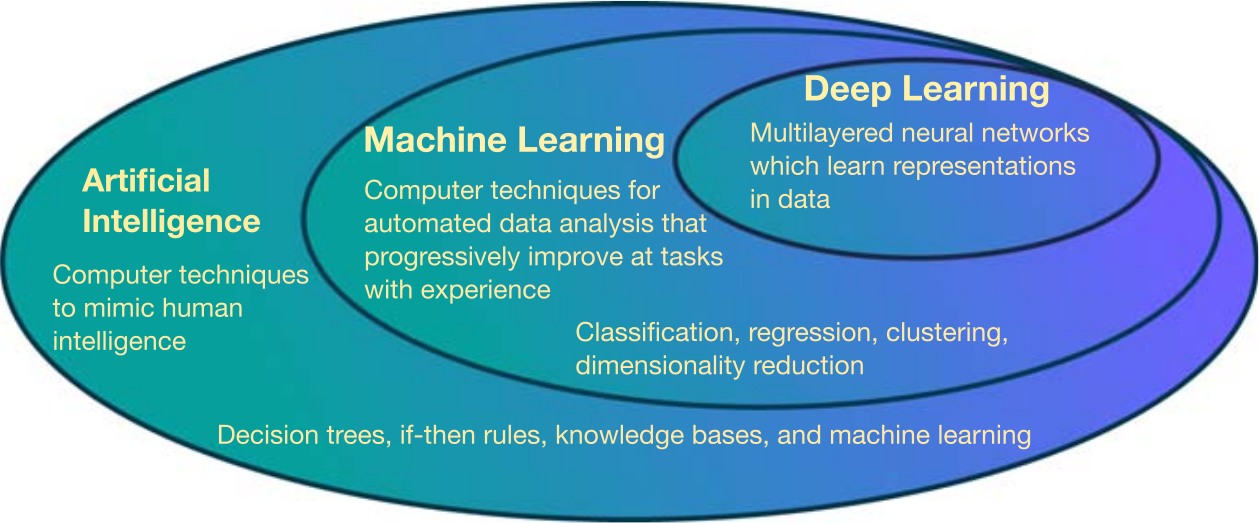
\includegraphics[height=1.9in,width=4.0in,viewport=0 0 1275 550,clip]{Figures/Hierarchical_description_AI_ML_DL.png}
\caption{\tiny{\textrm{Artificial Intelligence, Machine Learning and Deep Learning.}}}%
\label{AI-ML}
\end{figure}
}

\frame
{
	\frametitle{机器学习问题的一般形式与分类}
	\begin{itemize}
		\item 机器学习类问题的一般表示:
\vskip 5pt
对于给定的集合$\mathbf{X}$,可以预测或近似得到未知函数$y=f(\mathbf{X})$
\vskip 4pt
{\fontsize{6.2pt}{4.2pt}\selectfont{
	集合$\mathbf{X}$构成特征空间,集合中的每个元素$\mathbf{x}$称为特征向量(在材料类的机器学习中也称描述符)\\
	根据机器学习得到的近似函数$\hat{y}=\hat{f}(\mathbf{X})$,模型有能力预测训练数据之外的输出值}}
\vskip 5pt
	\textcolor{blue}{\fontsize{8.0pt}{4.2pt}\selectfont{机器学习的这种预测能力也称为模型的“泛化”\textrm{(generalization)}}}
\item 机器学习主要根据学习的特征分为无监督学习\textrm{(unsupervised learning)}和监督学习\textrm{(supervised learning)}
	\item 此外的机器学习问题还包括:~
\begin{itemize}
	\item 半监督学习,即大部分没有映射关系的数据和少量有映射关系的数据;
	\item 多任务和迁移学习,即将从相关问题习得的知识应用到数据极少的对象,提升模型的学习能力
	\item 强化学习,即没有输入输出,但会和环境不断交互,通过最大化环境的反馈,最终达到学习目标
\end{itemize}
	\end{itemize}
}

\frame
{
	\frametitle{机器学习问题的一般形式与分类}
\begin{figure}[h!]
\centering
\vspace*{-7pt}
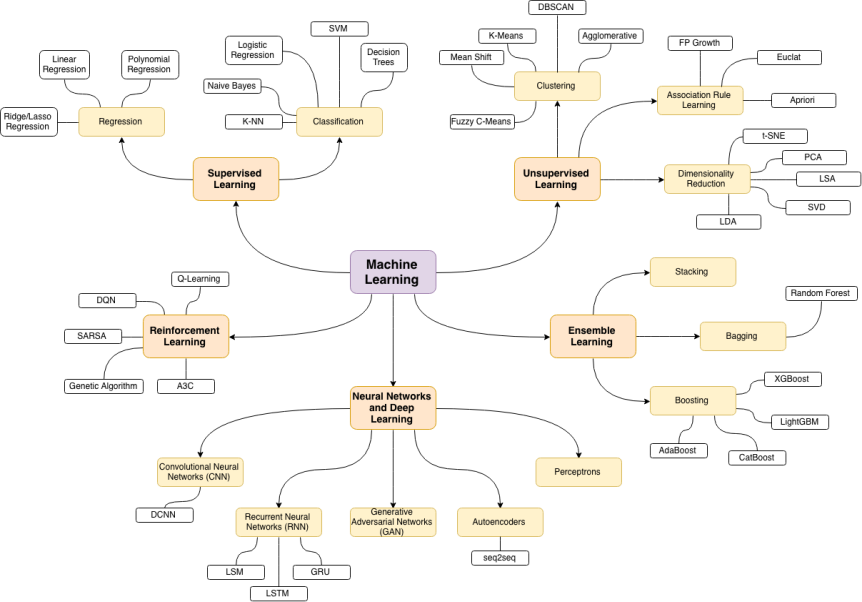
\includegraphics[height=2.7in,width=4.0in,viewport=0 0 875 620,clip]{Figures/ML_class.png}
%\caption{\fontsize{6.5pt}{4.5pt}\selectfont{面向多尺度材料智能计算平台}}%
\label{ML_classification}
\end{figure}
}

\frame
{
	\frametitle{数据挖掘的基本决策}
\begin{itemize}
	\item \textcolor{blue}{聚类}:~无指导的学习
	\item \textcolor{blue}{分类}:~有指导的学习
\end{itemize}
分类是数据挖掘的重要任务
\vskip 2pt
分类的\textcolor{red}{目的}:~机器学会分类函数或分类模型(称为分类器),通过模型能将数据库中的数据映射到特定类别中的某一类

\begin{figure}[h!]
\centering
\vspace*{-7pt}
\animategraphics[autoplay, loop, width=4.05in, height=1.55in]{15}{Figures/DNN-}{0}{15}
%\caption{\fontsize{6.5pt}{4.5pt}\selectfont{面向多尺度材料智能计算平台}}%
\label{ML_classification-animate}
\end{figure}
}

\frame
{
	\frametitle{无监督学习}
无监督学习是描述性质的,所有数据只有特征向量,没有标签,但呈现出聚群的结构,相似类型或特征的数据会聚集在一起
\begin{itemize}
	\item 如果没有标签的数据的组合是有限个,称为聚类\textrm{(clustering)};~无限的称为密度估计\textrm{(density estimation)}
	\item 将高维数据投影到低维空间,称为降维\textrm{(dimensionality reduction)}
		\vskip 2pt
		{\fontsize{8.0pt}{4.2pt}\selectfont{降维有助于了解复杂数数据的检测模式}}
%	\item 识别数据中的异常点或离群点
%		\vskip 2pt
%		{\fontsize{8.0pt}{4.2pt}\selectfont{异常检测可用于欺诈检测、故障预警等场景}}
\end{itemize}
\begin{figure}[h!]
\centering
\vspace*{-0.1in}
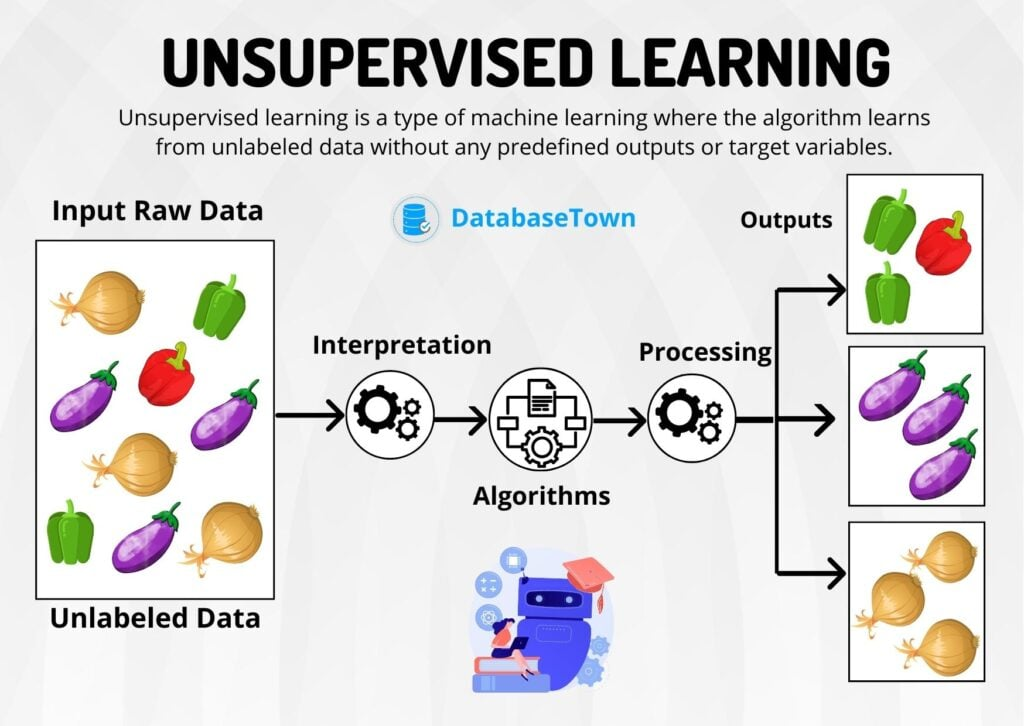
\includegraphics[height=1.5in,width=2.7in,viewport=0 0 1075 720,clip]{Figures/ML_Unsupervised-Learning.jpg}
\caption{\tiny{\textrm{The Schematic diagram of Unsupervised Learning.}}}%
\label{ML_Unsupervised-Learning}
\end{figure}
}

\frame
{
	\frametitle{监督学习}
	监督学习是通过学习指定数量的输入输出间的函数映射
\begin{itemize}
	\item 如果输出函数$y_{\mathrm{i}}$表示类别的有限集合,称为分类\textrm{(classification)}问题
		\vskip 2pt
		{\fontsize{8.0pt}{4.2pt}\selectfont{模型可用来预测未知数据所属类型}}
	\item 如果输出函数$y$是实数,称为回归\textrm{(regression)}问题
		\vskip 2pt
		{\fontsize{8.0pt}{4.2pt}\selectfont{模型可用来预测未知输入数据对应的值输出值}}
\end{itemize}
\begin{figure}[h!]
\centering
\vspace*{-0.1in}
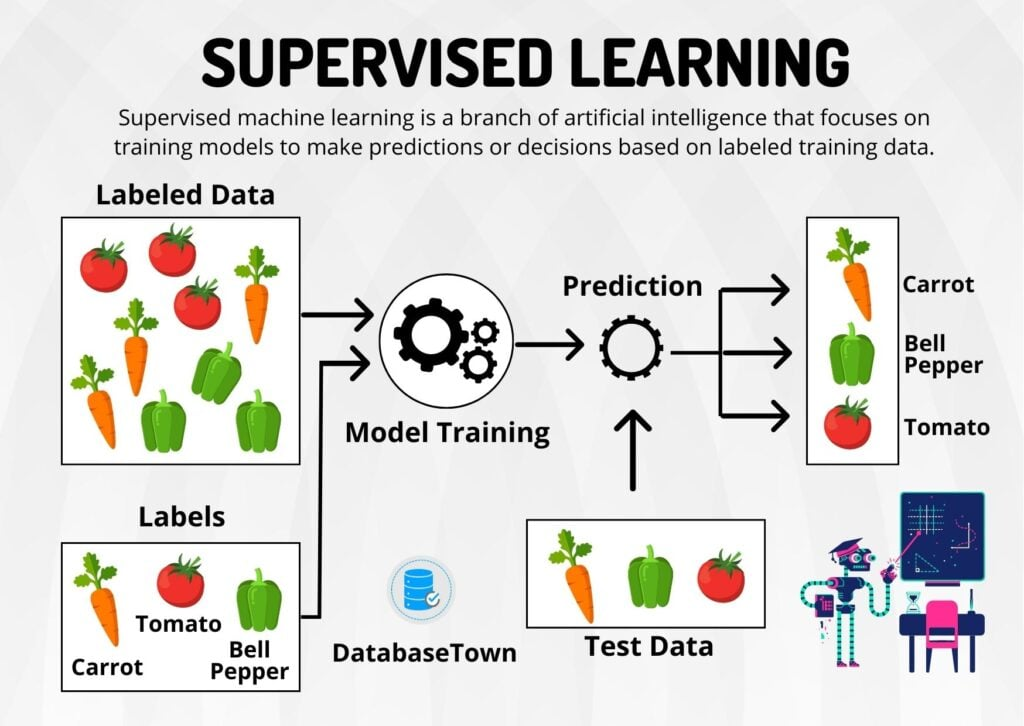
\includegraphics[height=1.6in,width=2.8in,viewport=0 0 1075 720,clip]{Figures/ML_Supervised-Learning-2.jpg}
\caption{\tiny\selectfont{\textrm{The Schematic diagram of Supervised Learning.}}}%
\label{ML_Supervised-Learning}
\end{figure}
}

\frame
{
	\frametitle{机器学习的流程}
\begin{itemize}
	\item \textcolor{blue}{数据的收集和筛选}:~{\fontsize{8.0pt}{4.2pt}\selectfont{从现有数据中产生并选择与问题解决有用和相关的数据子集}}
	\item \textcolor{blue}{数据预处理}:~清洗缺失和不完整数据,将数据将转换成统一的格式{\fontsize{8.0pt}{4.2pt}\selectfont{(如整型、字符串型等)}}%。必要时还须根据需要将数据按问题的格式重新表示
	\item \textcolor{blue}{数据训练}:~将数据分为训练集、验证集和测试集三部分,训练集数据用于学习并得到模拟参数{\fontsize{8.0pt}{4.2pt}\selectfont{(主要针对监督学习)}}
	\item \textcolor{blue}{模型测试和优化}:~用验证集数据评估模型的效果和性能,并用验证集数据优化模型
		\vskip 3pt
		{\fontsize{8.0pt}{4.2pt}\selectfont{一旦完成优化,用测试集数据评定模型的性能}}%。如果学习不成功,选用改善的数据重复上述步骤或改变学习算法。
	\item \textcolor{blue}{模型应用}:~将得到的有效模型对未知数据进行预测,如果有新的数据,模型还可以继续训练
\end{itemize}
}

\section{机器学习算法}
\frame
{
	\frametitle{主成分分析\textrm{(principal component analysis)}}
	主成分分析:\\
	{\fontsize{8.0pt}{4.2pt}\selectfont{\textcolor{blue}{将高维数据投影到数据点集中的区域,并使数据在新轴向周围聚集度最高}}}
{\fontsize{8.0pt}{4.2pt}\selectfont{
	\begin{itemize}
		\item 确定主成分:~找到$\mathbf{X}^T\mathbf{X}$的最大本征值对应的本征矢量(称为主成分)
			\vskip 1.5pt
			{\fontsize{7.0pt}{4.2pt}\selectfont{$\mathbf{X}$是已知高维数据集构成的矩阵}}
		\item 数据投影:~计算所有数据点对主成分的投影,实现数据压缩
		\item 局限:~ 假设数据位于线性子空间中
			\vskip 1.5pt
			{\fontsize{7.0pt}{4.2pt}\selectfont{只能为线性数据提供最佳结果}}
	\end{itemize}}}
\begin{figure}[h!]
\centering
\vspace*{-0.1in}
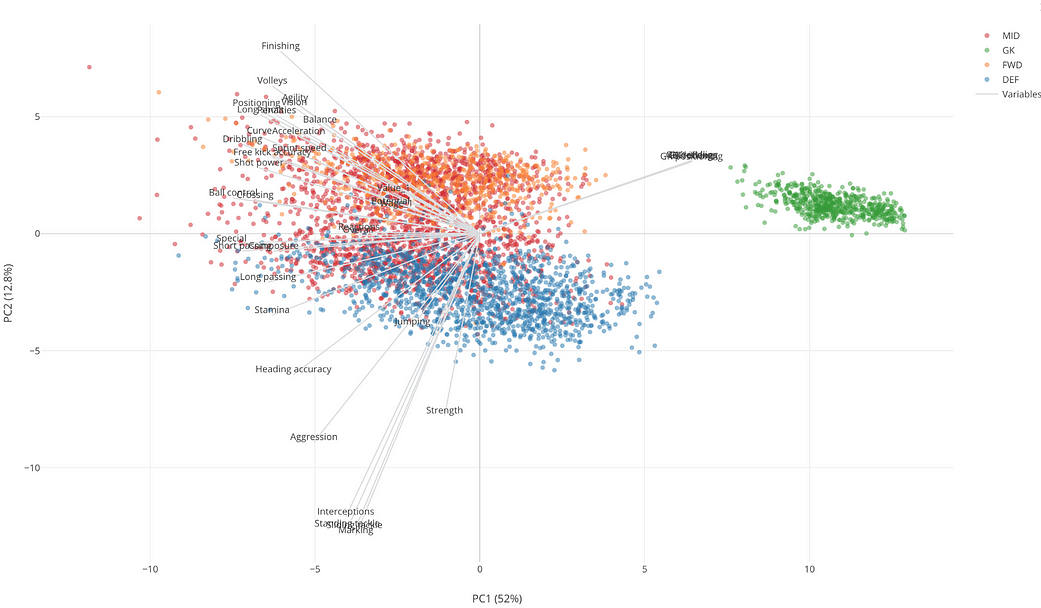
\includegraphics[height=1.70in,width=2.9in,viewport=0 0 1040 620,clip]{Figures/ML_PCM.png}
\caption{\tiny{\textrm{The Schematic diagram of Principal component analysis.}}}%
\label{ML_PCM}
\end{figure}
}

\frame
{
	\frametitle{$k$-\textrm{means}算法}
	$k$-\textrm{means}算法:~{\fontsize{8.0pt}{4.2pt}\selectfont{\textcolor{blue}{直接计算数据点和聚类中心的欧氏距离\textrm{(Euclidean distance)},将$n$个数据分类为$k$个子集($k<n$)}}}
	\vskip 3pt
{\fontsize{8.0pt}{4.2pt}\selectfont{
随机选定聚类中心的个数($k$)和位置($\mathbf{\mu}_0^{(\mathrm{j})}$,$1\leqslant j \leqslant k$),执行迭代:~
\begin{itemize}
	\item 计算每个数据点与聚类中心的距离,标记为$y_t^{\mathrm{(i)}}~(t>0)$,将该点分到距离最小的聚类中心所属的类中
		\begin{displaymath}
			y_t^{(\mathrm{i})}=\textrm{argmin}_j\|\mathbf{x}^{(\mathrm{i})}-\mu_t^{(\mathrm{j})}\|_p
		\end{displaymath}
	\item 重新计算每个聚类的中心$(\{\mu_t^{(\mathrm{j})}\})$
		\begin{displaymath}
			\mu_{t+1}^{(\mathrm{j})}=\dfrac1{n_j}\sum_{i=1}^{n_j}\mathbf{x}^{(\mathrm{i})}\delta_{y_t^{(\mathrm{i})},\mathrm{j}}
		\end{displaymath}
		$p\in\mathbb{N}$表示空间的维度(当$p=2$即为是二维平面的欧氏距离),$n_j$是归入聚类中心$\mu_t^{(\mathrm{j})}$的分类元素数目,$\delta_{n,m}$表示$\Delta$函数,$t$表示迭代次数
\end{itemize}
当标记不再变化时,迭代收敛}}
}

\frame
{
	\frametitle{$k$-\textrm{means}算法}
\begin{figure}[h!]
\centering
\vspace*{-0.1in}
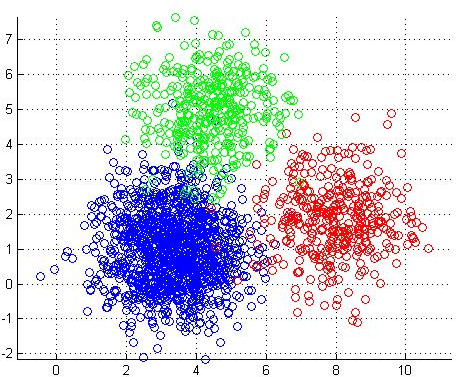
\includegraphics[height=1.80in,width=2.2in,viewport=0 0 110 90,clip]{Figures/ML_k-mean.png}
\caption{\tiny{\textrm{The Schematic diagram of the $k$-means algorithm.}}}%
\label{ML_k-means}
\end{figure}
$k$-\textrm{means}聚类算法的结果与初始聚类中心位置的选择密切关联
\vskip 3pt
{\fontsize{8.0pt}{4.2pt}\selectfont{初始聚类中心选择得不同,结果差别会比较大\footnote{\fontsize{6.0pt}{4.2pt}\selectfont{一般克服的策略是通过多次初始聚类中心并执行该算法,选择最有代表性的聚类形式作为结果}}}}
}

\frame
{
	\frametitle{层次聚类\textrm{(Hierarchical Clustering)}算法}
	层次聚类:~{\fontsize{8.0pt}{4.2pt}\selectfont{\textcolor{blue}{通过一层一层的进行聚类}}}
	\vskip 2pt
	{\fontsize{7.0pt}{4.2pt}\selectfont{\textcolor{magenta}{分裂法}:~由上向下把大的类别分割\\
	\textcolor{magenta}{聚合法}:~由下向上对小的类别聚合}}
{\fontsize{7.0pt}{4.2pt}\selectfont{
\begin{itemize}
	\item 初始时将每个训练数据点$\mathbf{x}^{(\mathrm{i})}$作为一个类(或类簇),原始类大小等于训练数据点数目$n$
	\item 衡量任意两个类(分别标记为\textrm{A}和\textrm{B})的偏差$d(\mathrm{A},\mathrm{B})$
	\item 偏差最小的两个类(最相似)合并一个新的类簇
\end{itemize}
反复执行该聚合过程,最终可以用一个类簇能囊括全部训练集}}
\begin{figure}[h!]
\centering
\vspace*{-0.04in}
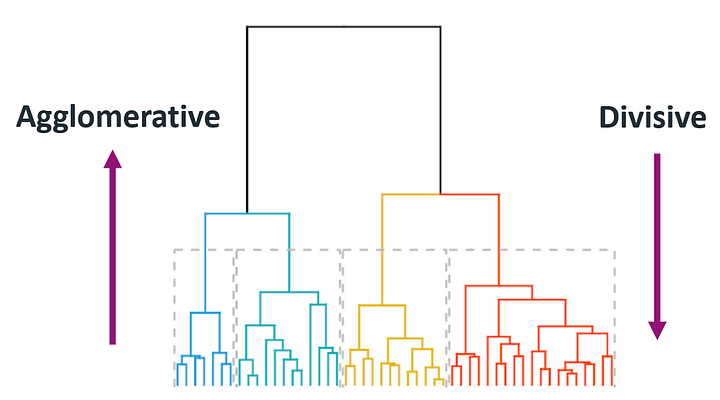
\includegraphics[height=1.47in,width=3.2in,viewport=0 0 730 390,clip]{Figures/ML_Hierarchical-Clustering.png}
\caption{\tiny{\textrm{The Schematic diagram of Hierarchical-Clustering algorithm.}}}%
\label{ML_ML_Hierarchical-Clustering}
\end{figure}
}

\frame
{
	\frametitle{层次聚类\textrm{(Hierarchical Clustering)}算法}
{\fontsize{8.0pt}{4.2pt}\selectfont{
要将$n$个类聚合成$k$个类簇~($1<k<n$)~,要在聚合中对聚合偏差设置截断,常见的聚合截断有三种:
\begin{itemize}
	\item 最小偏差
\begin{displaymath}
	d_{\mathrm{SL}}(\mathrm{A},\mathrm{B})=\min\limits_{i\in\mathrm{A},j\in\mathrm{B}}d_{ij}
\end{displaymath}
$d_{ij}$表示任意一对类的偏差
	\item 最大偏差
\begin{displaymath}
	d_{\mathrm{CL}}(\mathrm{A},\mathrm{B})=\max\limits_{i\in\mathrm{A},j\in\mathrm{B}}d_{ij}
\end{displaymath}
	\item 平均偏差
\begin{displaymath}
	d_{\mathrm{GA}}(\mathrm{A},\mathrm{B})=\dfrac1{|\mathrm{A}||\mathrm{B}|}\sum\limits_{i\in\mathrm{A}}\sum\limits_{j\in\mathrm{B}}d_{ij}
\end{displaymath}
\end{itemize}
定义的$d_{ij}$可以人为指定,对数值形式的数据,最常见的设置为欧氏距离}}
\vskip 5pt
分裂法与聚合法类似,只是初始时训练数据集属于一个类簇,然后逐层分裂形成特定的类簇
}

\frame
{
	\frametitle{线性回归\textrm{(Linear Regression)}算法}
对监督学习来说,每个数据不仅有特征向量$\mathbf{x}_{\mathrm{i}}$,还有相应的值$y_{\mathrm{i}}$
预测连续变化的$y$值,最常用的算法是线性回归
\vskip 3pt
{\fontsize{8.0pt}{4.2pt}\selectfont{回归算法的基本思想:~\textcolor{blue}{对于满足正态分布的数据点}
	\begin{itemize}
			\item 允许的参数拟合预测表达式
\begin{displaymath}
	\hat y^{(\mathrm{i})}=\theta^T\mathbf{x}^{(\mathrm{i})}
\end{displaymath}
{\fontsize{6.0pt}{4.2pt}\selectfont{上标$T$表示矢量的转置,$\hat y^{(\mathrm{i})}$是预测值,$\theta$是参数的矢量}}
		\item 为了求得$\theta$参数,定义误差的最小二乘函数
\begin{displaymath}
	J(\theta)=\sum_{i=1}^nL[\hat{y}^{(\mathrm{i})}(\mathbf{x}^{(\mathrm{i})},\theta),y^{(\mathrm{i})}]=\dfrac12\sum_{i=1}^n(\theta^T\mathbf{x}^{(\mathrm{i})}-y^{(\mathrm{i})})^2
\end{displaymath}
{\fontsize{6.0pt}{4.2pt}\selectfont{最小化该函数,可以得到最优化的参数$\theta$,由此可以得到线性回归机器学习的模型}}
\item 最优化参数$\theta$用矩阵表示可写作:~
\begin{displaymath}
	\theta=(\mathbf{X}^T\mathbf{X})^{-1}\mathbf{X}^T\mathbf{y}
\end{displaymath}
{\fontsize{6.0pt}{4.2pt}\selectfont{这里$\mathbf{X}$矩阵的每一列是由训练集输入数据$\mathbf{x}^{(\mathrm{i})}$,$\mathbf{y}$是对应的输出标注构成的矢量}}
	\end{itemize} }}
}

\frame
{
	\frametitle{预测模型的检验}
机器学习的模型性能,可用测试数据集检验,预测误差与训练数据集包含的数据数量密切相关:
\begin{itemize}
	\item 训练集数据不够,模型不能完全反映训练集特征\\
		{\fontsize{8.0pt}{4.2pt}\selectfont{预测结果将会表现出明显的偏差}}
	\item 训练集数据过多,模型能够体现训练集特征\\
		{\fontsize{8.0pt}{4.2pt}\selectfont{对训练集外的数据效果不好,出现过拟合\textrm{(overfitting)}}}
\end{itemize}
\begin{figure}[h!]
\centering
\vspace*{-0.1in}
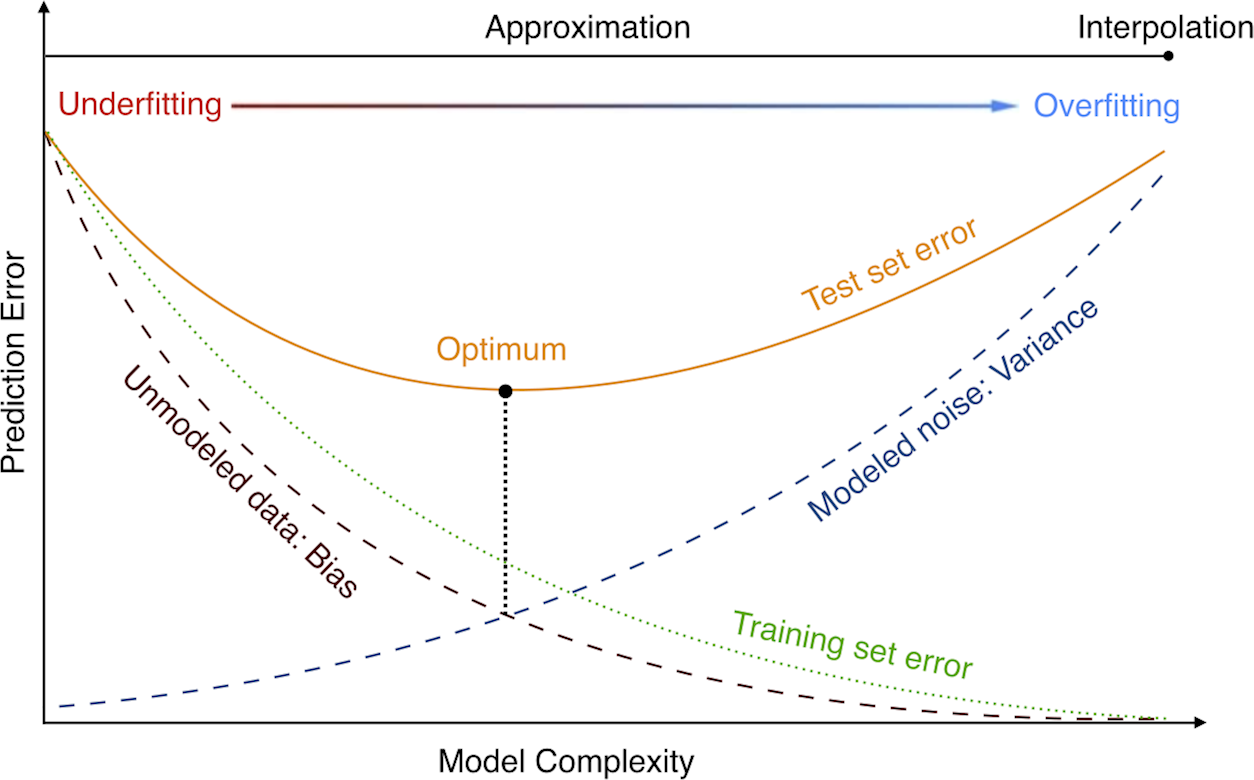
\includegraphics[height=1.4in]{The_optimum_comlexity_vs_prediction.png}
\caption{\tiny{\textrm{Complexity of the model:~Effective number of degrees of freedom (mainly tuned by the hyperparameters of the estimator).}}}%
\label{ML_Fitting_Error}
\end{figure}
}

\frame
{
	\frametitle{预测模型的检验}
回归算法的发展:~构建模型时,通过引入标准化参数$\lambda$来反应训练集元素变化的影响
\begin{displaymath}
	J(\theta)=\dfrac12\sum_{i=1}^n(\theta^T\mathbf{x}^{(\mathrm{i})}-y^{(\mathrm{i})})^2+\lambda\|\theta\|_p
\end{displaymath}
{\fontsize{7.0pt}{4.2pt}\selectfont{这里$p$表示数据度量形式}}
\vskip 4pt
{\fontsize{8.0pt}{4.2pt}\selectfont{优化参数$\lambda$降低训练集数据数量的影响:
	\vskip 3pt
	\textcolor{magenta}{通过压制或筛选训练数据集中的特征来调节其对误差函数的贡献}
\begin{itemize}
	\item $p=1$:~\textrm{Ridge Regression}
	\item $p=2$:~\textrm{LASSO Regression} 
\end{itemize}
\vskip 4pt
注意:~$\lambda$不能像$\theta$一样被优化}}
\vskip 2pt
{\fontsize{6.0pt}{4.2pt}\selectfont{一般是通过比较几个不同的$\lambda$值,选其中能最大化预测能力又不会引入太大偏差的一个}}
}

\frame
{
	\frametitle{分类算法:~逻辑回归\textrm{(logistic regression)}}
	逻辑回归,{\fontsize{8.0pt}{4.2pt}\selectfont{\textcolor{blue}{可以类比为映射到区间$[0,1]$之间的线性回归}}}: 
	\vskip 2pt
\begin{minipage}[b]{0.55\textwidth}
{\fontsize{7.0pt}{4.2pt}\selectfont{对于给定数据点$\mathbf{x}^{(i)}$,
\begin{itemize}
	\item $y^{(i)}=1$:~将其分入特定的“是\textrm{(True)}”类
	\item $y^{(i)}=0$:~将其分入特定的“否\textrm{(False)}”类
\end{itemize}
预测函数可以表示为
\begin{displaymath}
	\hat y=\sigma(\theta^T\mathbf{x})=\dfrac1{1+\mathrm{e}^{-\theta^T\mathbf{x}}}
\end{displaymath}
{\fontsize{5.0pt}{4.2pt}\selectfont{这里$\theta$仍是参数矢量,$\sigma$是逻辑函数(或 \textrm{sigmoid}函数)}}
\vskip 2pt
预测函数也可以视为条件概率:~$\hat{y}=P(y=1|\mathbf{x},\theta)$}}
\end{minipage}
\hfill
\begin{minipage}[b]{0.43\textwidth}
\begin{figure}[h!]
\centering
\vspace*{-0.4in}
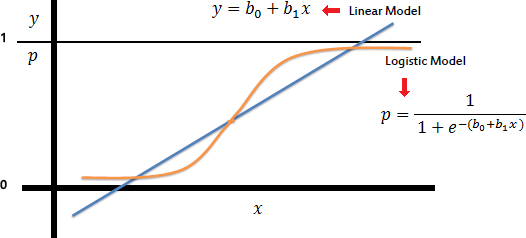
\includegraphics[height=0.75in]{ML_LR-LogReg.png}
%\caption{\tiny{\textrm{The Schematic diagram of linear model vs logistic model.}}}%
\label{ML_LR-LogReg}
\end{figure}
\end{minipage}
\vskip 2pt
{\fontsize{6.0pt}{4.2pt}\selectfont{分类问题的误差函数可定义为负的$\log$-型函数(交互熵\textrm{cross-entropy}),同样通过参数$\theta$最小化该函数:
\begin{displaymath}
	J(\theta) = -\dfrac1n\sum_{i=1}^n[y^{(\mathrm{i})}\log(\hat{y}^{(\mathrm{i})})+(1-y^{(\mathrm{i})})\log(1-\hat{y}^{(\mathrm{i})})]
\end{displaymath}
{\fontsize{5.0pt}{4.2pt}\selectfont{这里$y^{(\mathrm{i})}$和$\hat{y}^{(\mathrm{i})}=\sigma(\theta^T\mathbf{x}^{(\mathrm{i})})$分别为实际和预测值}}
\vskip 1pt
和线性回归类似,也可以引入正则参数$\lambda$}}
\vskip 2pt
{\fontsize{7.0pt}{4.2pt}\selectfont{逻辑分类也可用于处理超过两类的数据分类:\\
%	\vskip 1pt
	\textcolor{blue}{训练有$n$个逻辑回归值的模型,每一类对应一个数值,每个数据分入概率值最高的类中}}}
}

\frame
{
	\frametitle{支持向量机\textrm{(Support Vector Machines)}}
	支持向量机:~{\fontsize{7.5pt}{4.2pt}\selectfont{\textcolor{blue}{最通用的分类算法}
\vskip 2pt
定义函数
\begin{displaymath}
	J(\theta)=C\sum_{i=1}^n[y^{(\mathrm{i})}\max(\theta^T\mathbf{x}^{(\mathrm{i})},0)+(1-y^{(\mathrm{i})})\max(-\theta^T\mathbf{x}^{(\mathrm{i})},0)]+\dfrac1n\sum_{i=1}^n\theta_i^2
\end{displaymath}
{\fontsize{6.0pt}{4.2pt}\selectfont{这里$C$是参数}}
\begin{itemize}
	\item 在约束条件$y^{(\mathrm{i})}(\theta^T\mathbf{x}^{(\mathrm{i})}+b)\leqslant1$下,对全部训练数据点$(\mathbf{x}^{(\mathrm{i})},y^{(\mathrm{i})})$实现$\|\theta\|^2$最小化
	\item 引入\textrm{Lagrangian}乘子最小化$\|\theta\|^2$,可根据测试数据$i$的值$y^{(\mathrm{i})}$($+1$或$-1$),确定数据所属的类
\end{itemize}}}
\begin{figure}[h!]
\centering
\vspace*{-0.1in}
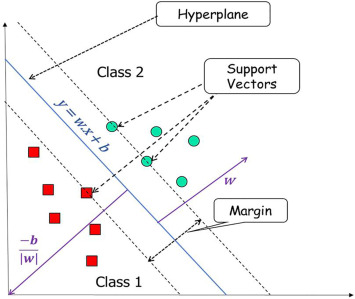
\includegraphics[height=1.4in,width=1.6in,viewport=0 0 230 190,clip]{ML_SVM.jpg}
\caption{\tiny{\textrm{The Schematic diagram of support vector machines algorithm.}}}%
\label{ML_SVM}
\end{figure}
}

\frame
{
	\frametitle{支持向量机\textrm{(Support Vector Machines)}}
	{\fontsize{7.5pt}{4.2pt}\selectfont{\textcolor{blue}{\textrm{SVM}最重要的特色是内核技巧\textrm{(kernel trick)}}\\
将参数矢量$\theta$用训练集数据表示
\begin{displaymath}
	\theta=\sum_i\alpha_iy^{(\mathrm{i})}\mathbf{x}^{(\mathrm{i})}
\end{displaymath}
因此可将分类规则写成数据点积的形式
\begin{displaymath}
	\theta^T\mathbf{x}+b=\sum_i\alpha_iy^{(\mathrm{i})}\mathbf{x}^{(\mathrm{i})}\cdot\mathbf{x}+b\leqslant0\rightarrow y=+1
\end{displaymath}
{\fontsize{6.0pt}{4.2pt}\selectfont{这里$b$和$\{\alpha_i\}$是待学习的参数}}
\vskip 2pt
\textcolor{blue}{内核技巧利用映射关系$\phi(\mathbf{x}):~\mathtt{R}^n\rightarrow\mathtt{R}^m$将矢量变换成$\mathbf{x}^{(\mathrm{i})}\cdot\mathbf{x}$点积}
\vskip 1pt
{\fontsize{6.0pt}{4.2pt}\selectfont{\textcolor{cyan}{实际上是将数据点映射到更高维度的空间中}}}
\vskip 2pt
所有矢量点积映射的变换都可以类似处理,最常用的内核
\begin{itemize}
	\item 多项式内核:
\begin{displaymath}
	K(\mathbf{x}^{(\mathrm{i})},\mathbf{x}^{(\mathrm{j})})=\phi(\mathbf{x}^{(\mathrm{i})})\cdot\phi(\mathbf{x}^{(\mathrm{j})})=(\mathbf{x}^{(\mathrm{i})}\cdot\mathbf{x}^{(\mathrm{j})}+1)^d,~d\in\mathtt{N}
\end{displaymath}
\item \textrm{Gaussian}内核(\textrm{radial basis function, RBF}内核)
\begin{displaymath}
	K(\mathbf{x}^{(\mathrm{i})},\mathbf{x}^{(\mathrm{j})})=\mathrm{e}^{\dfrac{-\|\mathbf{x}^{(\mathrm{i})},\mathbf{x}^{(\mathrm{j})}\|^2}{2\sigma^2}}
\end{displaymath}
\end{itemize}}}
}

\frame
{
	\frametitle{\textrm{Na\"ive~Bayes}分类}
{\fontsize{8.0pt}{4.2pt}\selectfont{
分类算法的判别模式
\begin{itemize}
	\item 基于判别模式\textrm{(discriminative model)}:~数据点预测的标签是条件概率$p(y|\mathbf{x})$
	\item 基于生成模式\textrm{(generative model)},预测点条件概率用后验\textrm{Bayes}公式表示
\begin{displaymath}
	p(y|\mathbf{x})=\dfrac{p(\mathbf{x}|y)p(y)}{p(\mathbf{x})}=\dfrac{p(\mathbf{x}|y)p(y)}{\sum\limits_ip(\mathbf{x}|y=i)p(y=i)}
\end{displaymath}
{\fontsize{6.0pt}{4.2pt}\selectfont{这里$p(y)$表示先验概率,即没有附加任何先期知识和分析得到的概率}}
\end{itemize}
\begin{minipage}[b]{0.59\textwidth}
假设数据点的特征向量$\mathbf{x}^{(\mathrm{i})}$和值$y^{(\mathrm{i})}$完全独立,可有\textrm{Na\"ive~Bayes}分类算法(后验概率):
\begin{displaymath}
	p(y|\mathbf{x})=\dfrac{\prod\limits_{j=1}^np(x_j|y)p(y)}{p(\mathbf{x})}
\end{displaymath}
{\fontsize{6.0pt}{4.2pt}\selectfont{这里$x_j$表示特征向量$\mathbf{x}$的元素}}%,这里主要讨论分子,因为分母先验概率$p(\mathbf{x})$是与$y$无关的常数且和是归一化的
\end{minipage}
\hfill
\begin{minipage}[b]{0.39\textwidth}
\begin{figure}[h!]
\centering
\vspace*{-0.05in}
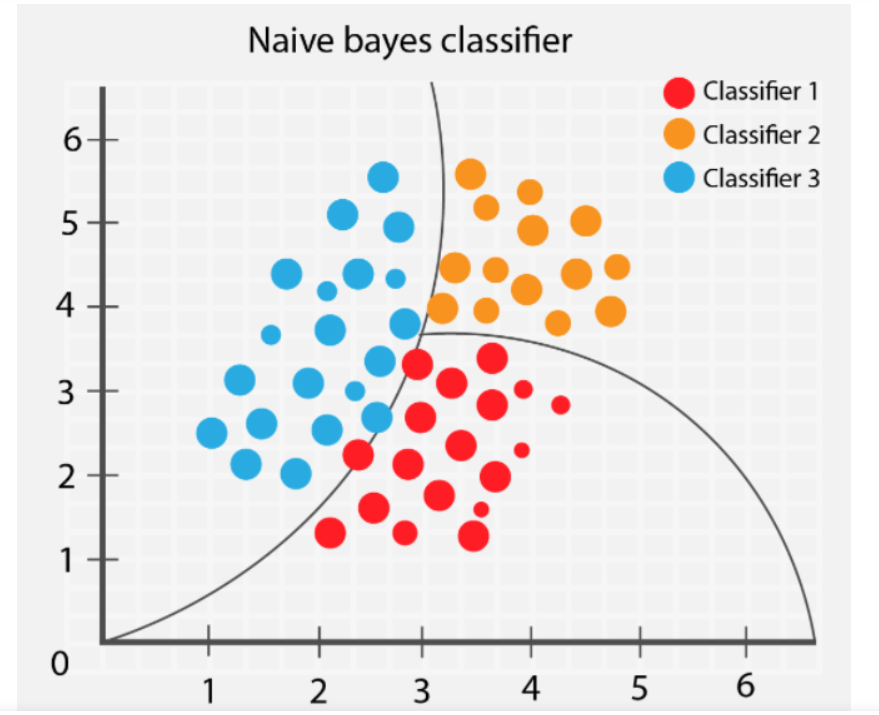
\includegraphics[height=1.2in,width=1.5in,viewport=0 0 550 470,clip]{ML_Naive-Bayes.png}
%\caption{\tiny{\textrm{The Schematic diagram of Na\"ive-Bayes algorithm.}}}%
\label{ML_NavieBayes}
\end{figure}
\end{minipage}
\begin{itemize}
	\item 分类前先列出训练数据点的全部先验概率$p(y)$和条件概率$p(x_j|y)$
	\item 用\textrm{Na\"ive~Bayes}算法计算后验概率
	\item 选择所有$y$中最大的后验概率$p(y|\mathbf{x})$作为分类预测值
\end{itemize}}}
}

\frame
{
	\frametitle{$k$-最近邻\textrm{($k$-nearest neighbors)}算法}
	$k$-最近邻算法:~{\fontsize{8.0pt}{4.2pt}\selectfont{\textcolor{blue}{利用数据点空间距离的类似性,不再训练,适合处理快速任务}
\vskip 3pt
	$d$-维空间有训练集数据$\{\mathbf{x}^{(\mathrm{i})}\}$,计算未知数据点与已知数据点之间的空间距离
\begin{displaymath}
	d(\mathbf{x},\mathbf{x}^{(\mathrm{i})})=\|\mathbf{x}-\mathbf{x}^{(\mathrm{i})}\|_p
\end{displaymath}
{\fontsize{6.0pt}{4.2pt}\selectfont{这里的$p$是维度参数}}
\vskip 3pt
一旦得到$\mathbf{x}$到空间各点的距离,$\mathbf{x}$点归入与其有最近邻$k$值最大的类中
\vskip 2pt
如果没有最大类,则随机归入最近邻点的最常使用的标注类中
\begin{itemize}
	\item 对连续值求平均,就是基于\textrm{k-NN}的回归
	\item $k$值的选取对于分类很敏感,不同的$k$值很可能得到完全不同的数据分类
\end{itemize}}}
\begin{figure}[h!]
\centering
\vspace*{-0.1in}
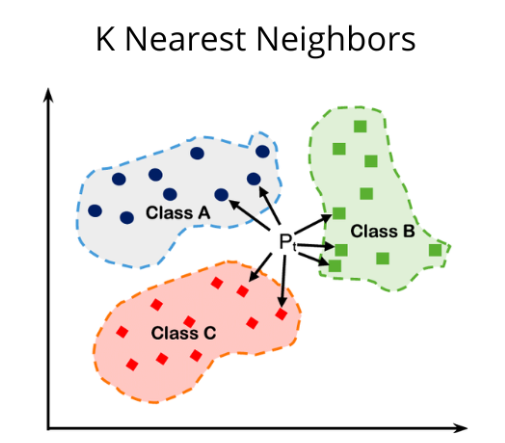
\includegraphics[height=1.5in,width=1.8in,viewport=0 0 530 450,clip]{ML_kNN-2.png}
\caption{\tiny{\textrm{The Schematic diagram of $k$-nearest neighbors algorithm.}}}%
\label{ML_k-NN}
\end{figure}
}

\frame
{
	\frametitle{决策树\textrm{(Decision Trees)}}
	决策树:~{\fontsize{8.0pt}{4.2pt}\selectfont{\textcolor{blue}{通过创建节点来实现对某种分裂算法的优化}
	\vskip 2pt
	\textcolor{magenta}{同时适合分类和回归}
	\begin{itemize}
		\item 决策树上每个节点都含一个定义该部分空间划分的方案,直到空间不可再分
		\item 每个不连通的子空间称为\textcolor{blue}{叶节点},叶节点包含了待分类或预测的数据点
	\end{itemize}
决策树的主要问题:~一旦开始训练,往往伴随过拟合}}
\begin{figure}[h!]
\centering
%\vspace*{-0.05in}
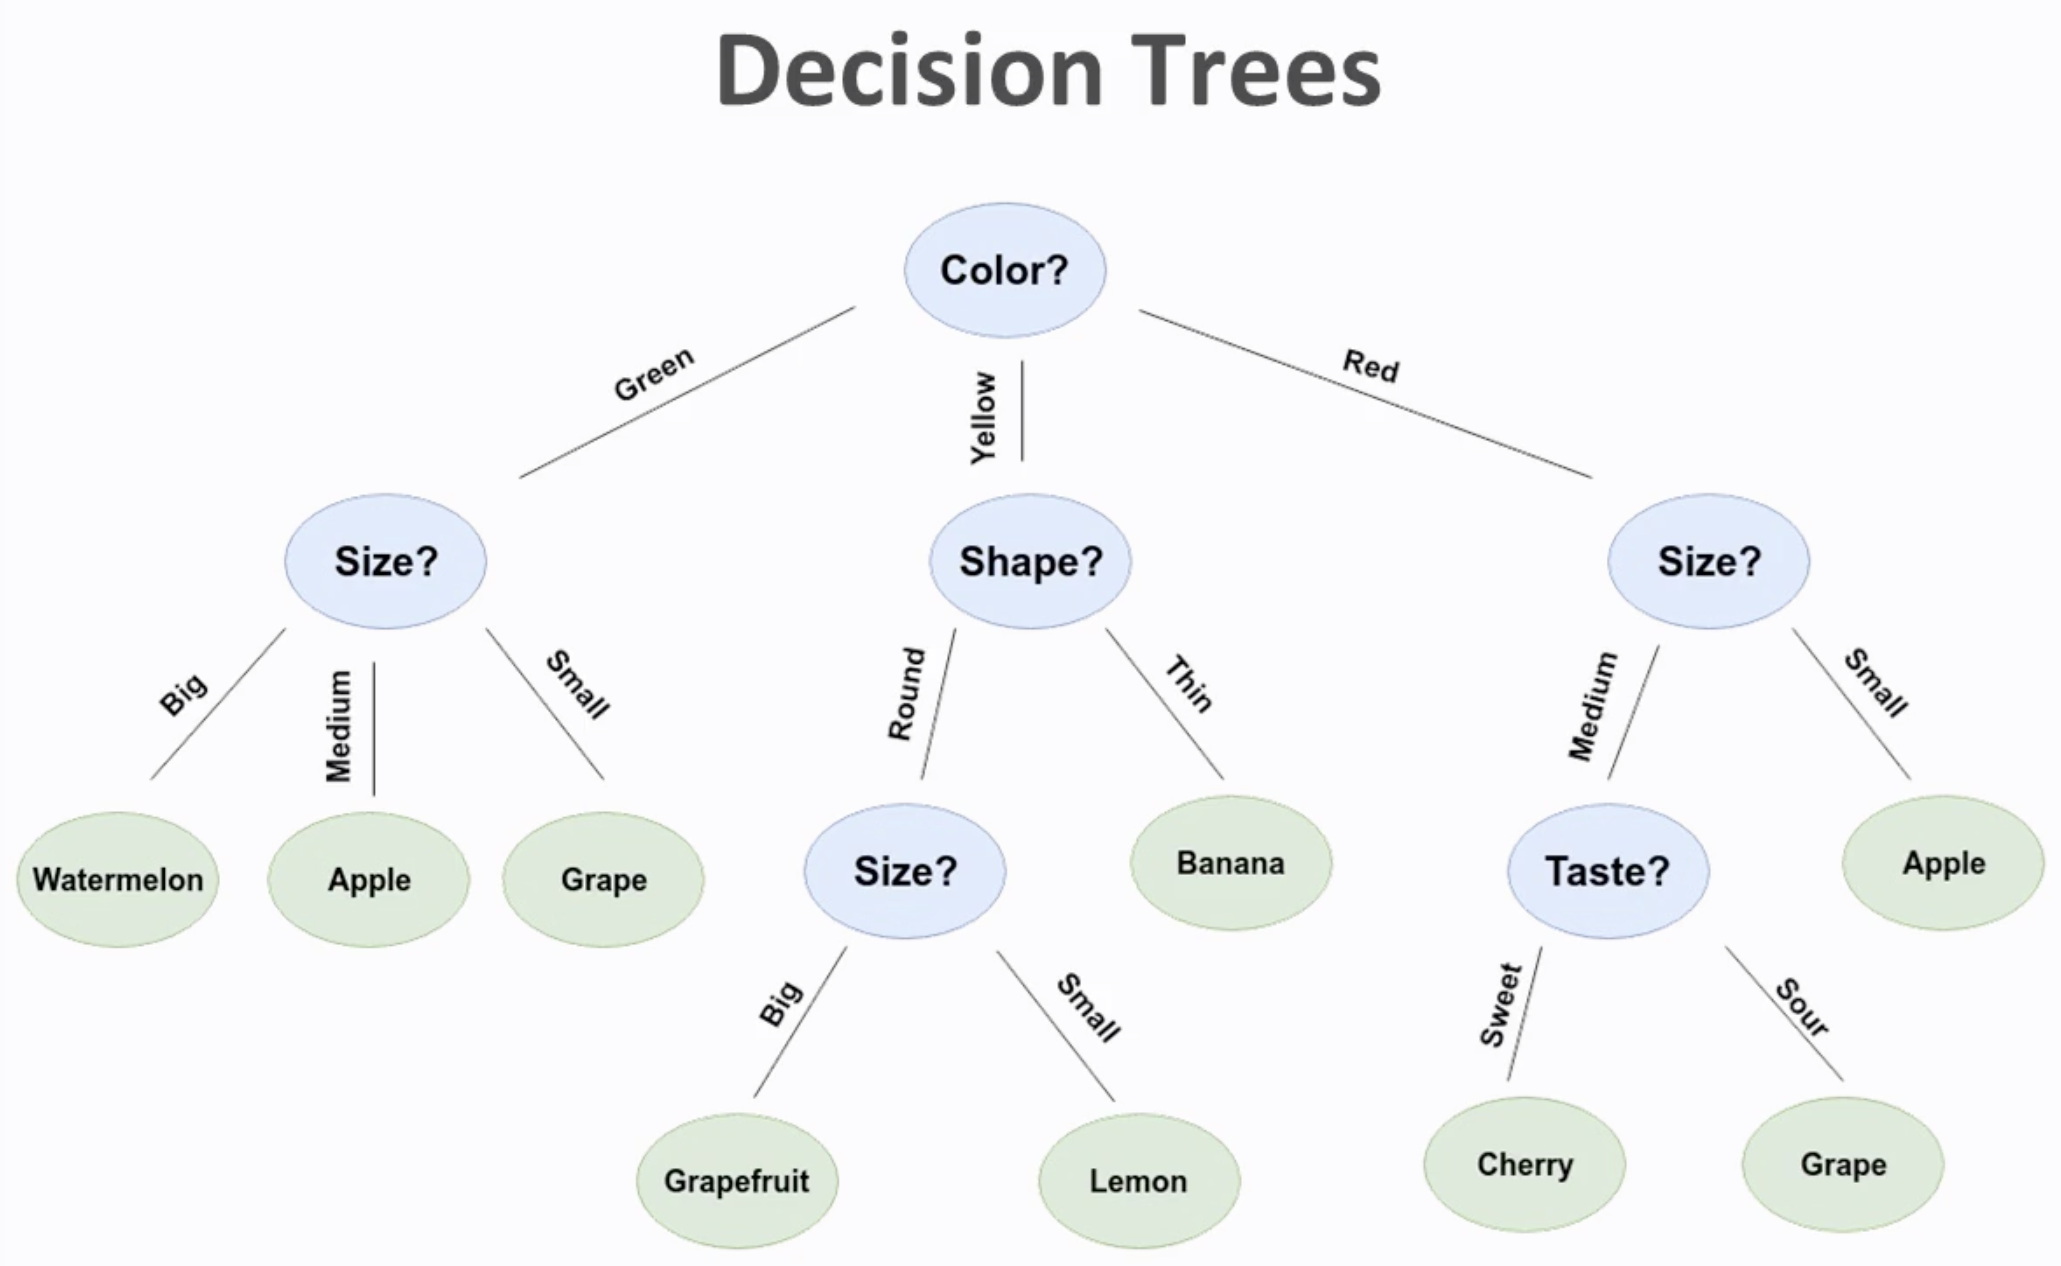
\includegraphics[height=1.95in,width=3.4in,viewport=0 0 2070 1250,clip]{ML_decision-trees.png}
\caption{\tiny{\textrm{The Schematic diagram of decision trees algorithm.}}}%
\label{ML_Decision-trees}
\end{figure}
}

\frame
{
	\frametitle{随机森林\textrm{(Random Forest)}}
{\fontsize{8.0pt}{4.2pt}\selectfont{克服决策树过拟合的策略:
\begin{itemize}
	\item 修剪决策树分叉,会损失一定的精度,但提高回归的泛化能力
	\item 采用随机森林,即训练大量的决策树然后再取统计平均值
\end{itemize}
随机森林方法是一种系综平均方法:~\textcolor{blue}{决策树将成为训练对象}
\vskip 2pt
对决策树的特征进行随机抽样训练时,一般采取自展抽样\textrm{(bootstrap sample)}方案
\begin{figure}[h!]
\centering
%\vspace*{-0.05in}
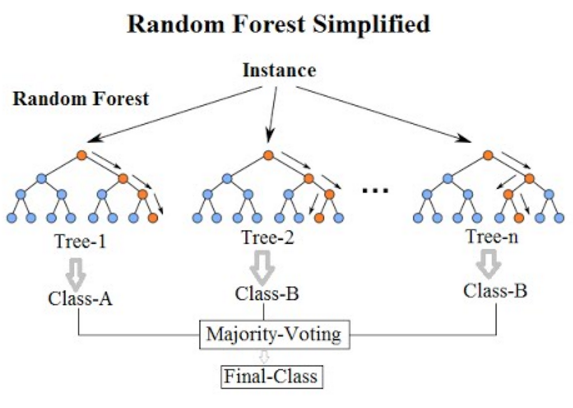
\includegraphics[height=2.00in,width=3.0in,viewport=0 15 570 400,clip]{ML_radom-forest.png}
\caption{\tiny{\textrm{The Schematic diagram of random forest algorithm.}}}%
\label{ML_Random-Forest}
\end{figure}
随机森林算法将一系列的非强化学习的功能组合起来,对未知数据有更好的预测能力}}
}

\frame
{
	\frametitle{深度神经网络基础}
{\fontsize{8.0pt}{4.2pt}\selectfont{
	\begin{itemize}
		\item 感知机(\textrm{Perceptron Learning Algorithm, PLA}):
			\vskip 3pt
			最早的监督式训练算法,是神经网络构建的基础
\begin{figure}[h!]
%\vspace*{-0.08in}
\centering
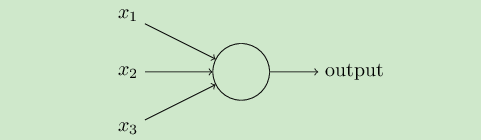
\includegraphics[height=0.50in]{Figures/DNN_PLA.png}
\caption{\tiny \textrm{Perceptron Learning Algorithm.}}%(与文献\cite{EPJB33-47_2003}图1对比)
\label{Fig:PLA}
\end{figure}
输出与输入之间将学习到一个线性关系,可有中间输出结果
\begin{displaymath}
	z=\sum_{i=1}^mw_ix_i+b
\end{displaymath}
中间结果连接一个神经元激活函数
\begin{displaymath}
	\mathrm{sign}(z)=\left\{
		\begin{aligned}
			-1\qquad &z<0\\
			1 \qquad &z\geqslant 0
		\end{aligned}\right.
\end{displaymath}
	\end{itemize}}}
}

\frame
{
	\frametitle{深度神经网络基础}
\begin{figure}[h!]
\vspace*{-0.08in}
\centering
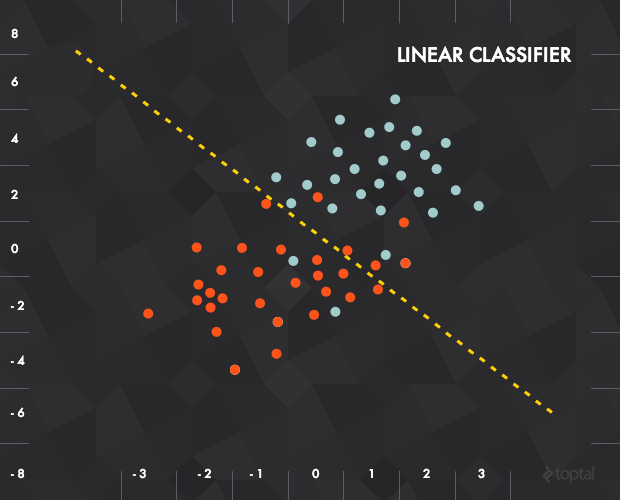
\includegraphics[width=2.5in]{Figures/NN_PLA_example.png}
%\caption{\tiny \textrm{Perceptron Learning Algorithm.}}%(与文献\cite{EPJB33-47_2003}图1对比)
\label{Fig:PLA}
\end{figure}
{\fontsize{8.0pt}{4.2pt}\selectfont{
\begin{itemize}
	\item 每一个输入数据都可以表示为一个向量$x = (x_1, x_2)$
	\item 函数则是要实现“如果线以下,输出0;线以上,输出1”
\end{itemize}}}
}

\frame
{
	\frametitle{深度神经网络基础}
{\fontsize{8.0pt}{4.2pt}\selectfont{
感知机模型只能用于二元分类,无法学习较为复杂的非线性模型,神经网络在感知机模型基础上作了扩展
%\vskip 10pt
	\begin{itemize}
		\item 加入隐藏层(\textrm{hide layer}):\\
			隐藏层可以有很多层,增强模型的表达能力
		\item 输出层的神经元可以有不止一个输出
		\item 对激活函数作扩展,如\textrm{Sigmoid}函数
			\begin{displaymath}
				f(z)=\dfrac1{1+\mathrm{e}^{-z}}
			\end{displaymath}
			{\fontsize{6.5pt}{4.2pt}\selectfont{其他的激活函数还有\textrm{tanx}、\textrm{softmax}和\textrm{ReLU}等}}
\begin{figure}[h!]
%\vspace*{-0.08in}
\centering
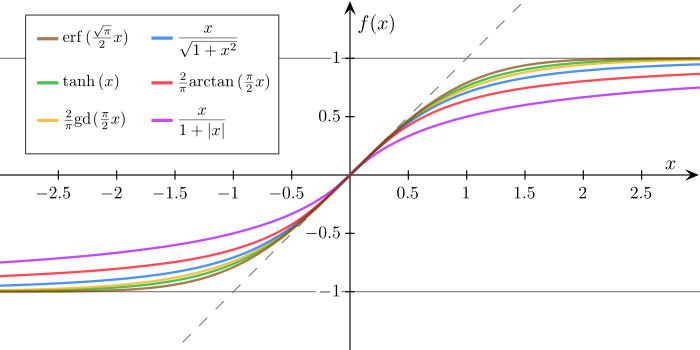
\includegraphics[width=2.8in]{Figures/ML_Sigmoid-Gjl-t.png}
%\caption{\tiny \textrm{Perceptron Learning Algorithm.}}%(与文献\cite{EPJB33-47_2003}图1对比)
\label{Fig:Sigmoid_curve}
\end{figure}
	\end{itemize}}}
}

\frame
{
	\frametitle{深度神经网络\textrm{(Deep Learning Neural Network)}}
{\fontsize{8.0pt}{4.2pt}\selectfont{
深度神经网络可以包含上百层神经元,通常有上万个参数,再加上超参数,实际的参数空间几乎是无限大的
\begin{figure}[h!]
%\vspace*{0.05in}
\centering
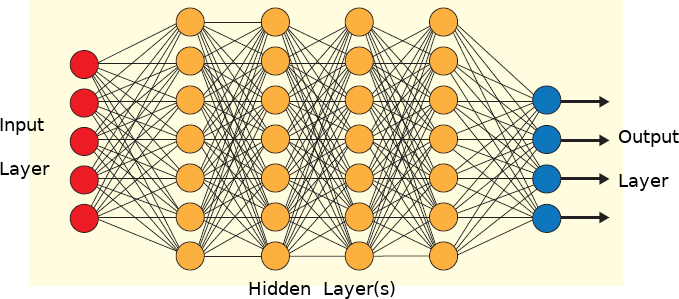
\includegraphics[height=1.90in,width=4.05in]{Figures/ANN_Algorithm.png}
\caption{\tiny \textrm{Deep Learning Neural Network.}}%(与文献\cite{EPJB33-47_2003}图1对比)
\label{Fig:Deep-Learning-NN}
\end{figure}
\textcolor{red}{如何从海量潜在的可能参数中做选择极具挑战性}}}
}

\frame
{
	\frametitle{深度神经网络的前馈算法}
	以三层深度神经网络为例,说明深度神经网络的前馈算法
\begin{figure}[h!]
%\vspace*{-0.08in}
\centering
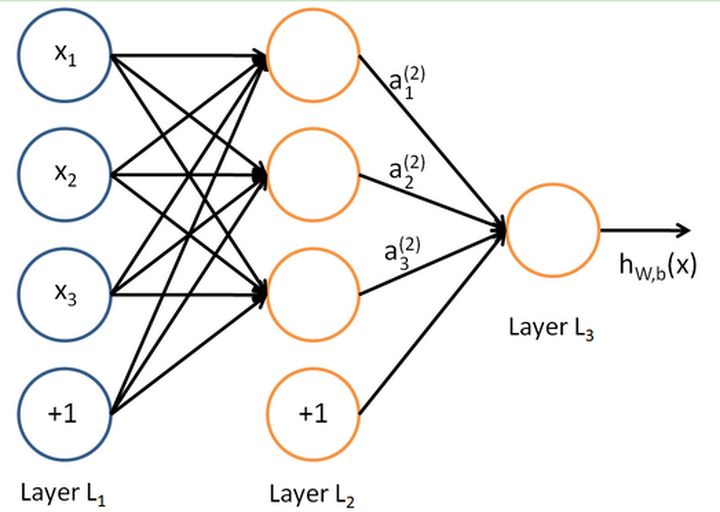
\includegraphics[width=3.0in]{Figures/DNN_front_pro.jpg}
%\caption{\tiny \textrm{Perceptron Learning Algorithm.}}%(与文献\cite{EPJB33-47_2003}图1对比)
\label{Fig:PLA}
\end{figure}
}

\frame
{
	\frametitle{遗传算法\textrm{(Genetic Algorithm)}}
{\fontsize{8.0pt}{4.2pt}\selectfont{
	遗传算法:~模拟生物进化论的自然选择和遗传学机理的计算模型
	\vskip 2pt
	\textcolor{blue}{通过模拟自然进化过程搜索最优解}
	\begin{enumerate}
		\item 优化问题可能潜在的解集构成一个种群(\textrm{population})
			\vskip 2pt
			该种群由经过基因(\textrm{gene})编码的一定数目的个体(\textrm{individual})组成,每个个体是染色体(\textrm{chromosome})带有特征的实体
%		\item 优化问题可能潜在的解集构成一个种群,该种群由经过基因编码的一定数目的个体组成,每个个体是带有一定的优化特征
		\item 种群产生之后,借助于自然遗传学的遗传算子(\textrm{genetic operators})进行组合\\
			交叉(\textrm{crossover})和变异(\textrm{mutation}),产生新一代个体
%		\item 种群产生之后,借助于自然遗传学的遗传算子进行组合交叉(\textrm{crossover})和变异(\textrm{mutation}),产生新一代个体
\begin{figure}[h!]
\vspace*{-0.05in}
\centering
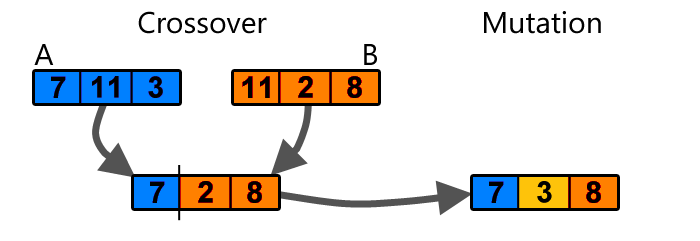
\includegraphics[width=2.7in]{Figures/Genetic_Algorithm_basic.png}
%\caption{\tiny \textrm{Perceptron Learning Algorithm.}}%(与文献\cite{EPJB33-47_2003}图1对比)
\label{Fig:PLA}
\end{figure}
		\item 适者生存和优胜劣汰:~在每一代,根据问题计算个体的适应度(\textrm{fitness})
			\vskip 2pt
			选择(\textrm{selection})合适的个体,构成代表新的解集的种群
\vspace*{-0.10in}
%		\item 按照适者生存和优胜劣汰的原理,在每一代,根据问题域中个体的适应度,选择合适的个体,构成代表新的解集的种群
		\item 逐代(\textrm{generation})演化后,产生出越来越好的近似解(优化目标)
%		\item 逐代演化后,产生出越来越好的近似解(优化目标)
	\end{enumerate}}}
}

\frame
{
	\frametitle{深度神经网络与遗传算法}
	\textcolor{blue}{深度神经网络类似问题的解决方案:~遗传算法}
\begin{minipage}[b]{0.49\textwidth}
	\vskip 10pt
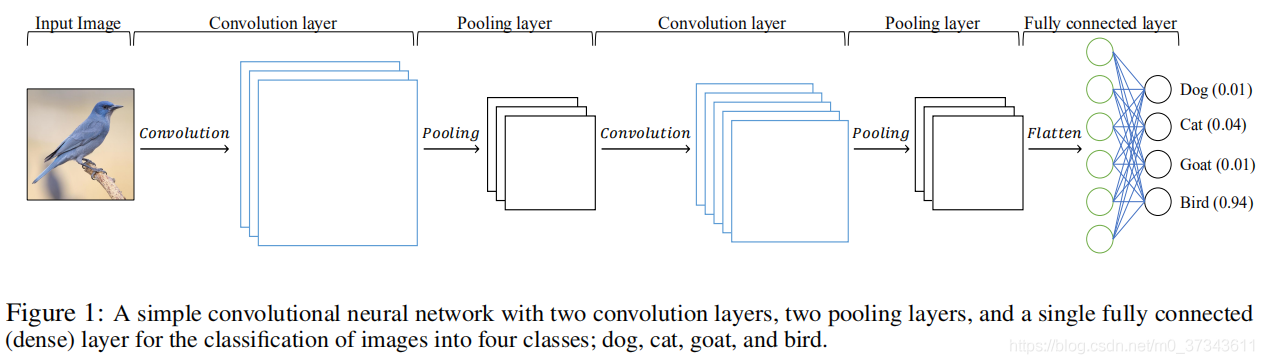
\includegraphics[height=0.4in,width=2.08in,viewport=0 110 1280 350,clip]{Figures/Genetic_Algorithm-2.png}\\
\centering{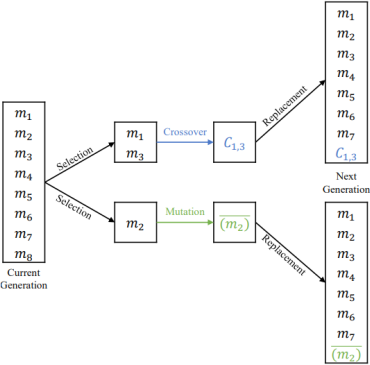
\includegraphics[height=1.0in,width=1.08in,viewport=140 50 820 650,clip]{Figures/Genetic_Algorithm-1.png}}\\
\vskip 0.02pt
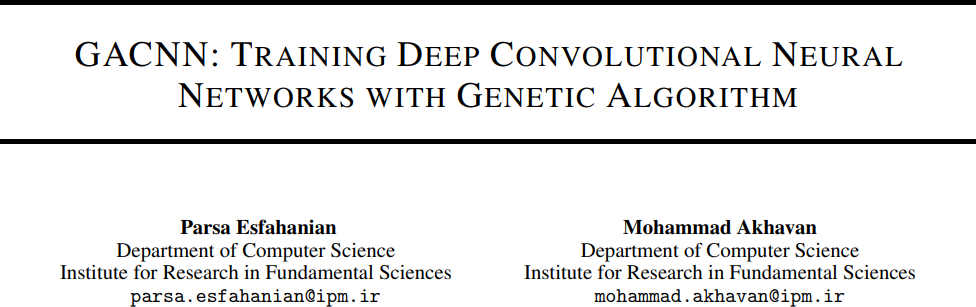
\includegraphics[height=0.7in,width=2.05in]{Figures/Genetic_Algorithm-3.png}\\
%\centering{\textcolor{red}{\textrm{\tiny GACNN:~利用遗传算法训练深度卷积神经网络}}}
\end{minipage}
\hfill
\begin{minipage}[b]{0.49\textwidth}
	\vskip 10pt
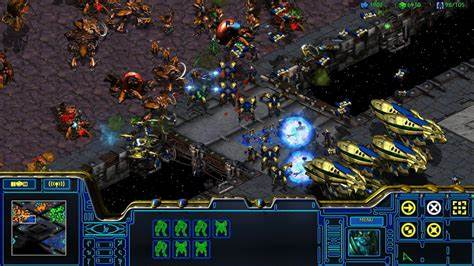
\includegraphics[height=1.2in,width=1.9in]{Figures/Genetic_Algorithm-5.png}\\
\vskip 0.5pt
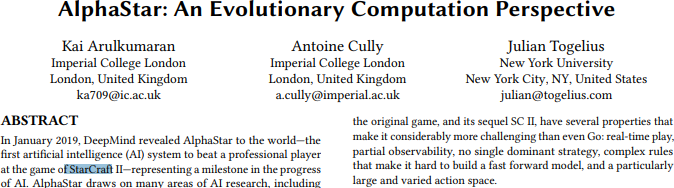
\includegraphics[height=0.55in,width=1.95in]{Figures/Genetic_Algorithm-4.png}\\
%\centering{\textcolor{red}{\textrm{\tiny 多智能体强化学习:~神经网络}}}
\end{minipage}
}

\frame
{
	\frametitle{机器学习的验证}
{\fontsize{8.0pt}{4.2pt}\selectfont{机器学习模型是否仅对训练数据有效,还需要一些数据集来检验\footnote{\fontsize{5.0pt}{4.2pt}\selectfont{模型对训练集的学习,优化的并非全部参数,以神经网络为例,网络隐藏层的数目作为参数在优化过程中就始终保持不变,这类参数称为超参数(\textrm{hyperpameter})。通过验证集检验的主要是模型中未能优化的超参数的性能}},这一过程称为验证,对应的数据集称为验证集
\begin{itemize}
	\item 监督学习的数据集一般分为三类:~训练集、验证集和测试集
		\vskip 2pt
	{\fontsize{6.0pt}{4.2pt}\selectfont{这些样本数据最好是具备相同的统计分布特征。为了优化学习模型,建议先对样本数据多次学习,最后才将模型应用到测试数据集上}}
\item 对比预测数据和实际数据的偏差,可以评估模型的真实预测能力
\item 当数据非常有限时,最常用的是\textcolor{blue}{~$k$-重交叉验证\textrm{(cross-validation)}}:
	\vskip 2pt
	{\fontsize{6.0pt}{4.2pt}\selectfont{将训练集分成$k$个子集,选择$k-1$个子集训练模型,并用剩下的一个未训练的子集验证模型:\\将训练-验证过程执行$K$次,并将$K$次验证的平均损失函数来评估模型性能的平均表现
\vskip 1pt
	平均损失函数定义为:
\begin{displaymath}
	E_{\mathrm{cv}}^{K}=\dfrac1K\sum_{k=1}^K\sum_{i=1}^{n_k}L(\hat{y}_k^{(\mathrm{i})},y^{(\mathrm{i})})
\end{displaymath}
{\fontsize{5.0pt}{4.2pt}\selectfont{这里$L$是验证数据集的损失函数,$\hat{y}_k^{(\mathrm{i})}$是训练子集(不含验证子集$k$)得到的模型,对采样数据$i$预测的值$\hat{y}_k^{(\mathrm{i})}$,训练子集的采样数据共有$n_k$}}\\
特别地,$K=n$,即训练集划分的子集与其元素个数相同,称为\textrm{leave-one-out cross-validation}}}
\end{itemize}
{\fontsize{7.0pt}{4.2pt}\selectfont{\textcolor{purple}{交叉验证也可用于评估训练模型中的超参数}\footnote{\fontsize{5.0pt}{4.2pt}\selectfont{超参数包括正则化参数$\lambda$、\textrm{S\!V\!M}的\textrm{Gaussian}内核参数$\sigma$,二叉树(二元决策)修剪层次和随机森林系综的特征向量等}}:~选择有最小的预测误差时的参数}}}}
}

\frame
{
	\frametitle{机器学习的验证}
	{\fontsize{8.0pt}{4.2pt}\selectfont{对机器学习模型性能的评估手段有很多
		\begin{itemize}
			\item 二元或多元分类可以选用\textcolor{blue}{混同矩阵\textrm{(confusion matrices)}}\footnote{\fontsize{5.0pt}{4.2pt}\selectfont{所谓混同矩阵,就是评估模型预测与抽样吻合程度建立的矩阵,预测吻合度高的元素主要出现在矩阵对角元,预测吻合度低的都在矩阵非对角元}}
				\vskip 2pt
				{\fontsize{5.0pt}{4.2pt}\selectfont{比如矩阵的列方向为采用数据的值,行方向是预测数据的值(除了近似单位矩阵表示,也可以用真阳\textrm{(TP)}、真阴\textrm{(TN)}和假阳\textrm{(FP)}假阴\textrm{(FN)}来填充矩阵)}}
			\item 绘制模型\textcolor{blue}{受试操作特征\textrm{(receiver operating characteristic, ROC)}曲线}\\
				{\fontsize{5.0pt}{4.2pt}\selectfont{也可以用比如“真阳率”\textrm{(TP rate)}~$\mathrm{TPR}=\frac{\mathrm{TP}}{\mathrm{TP}+\mathrm{FN}}$和“假阳率”\textrm{(FP rate)}~$\mathrm{FPR}=\frac{\mathrm{FP}}{\mathrm{FP}+\mathrm{TN}}$}}
		\end{itemize}
\begin{figure}[h!]
\centering
\vspace*{-0.1in}
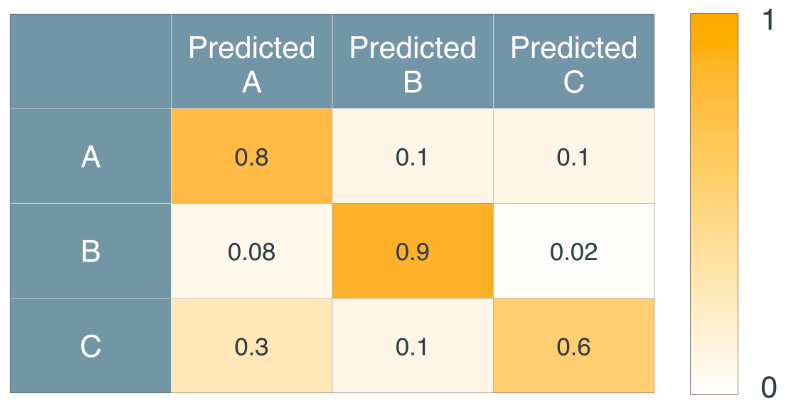
\includegraphics[height=1.2in]{ML_confusion_matrix.png}
\hskip 5pt
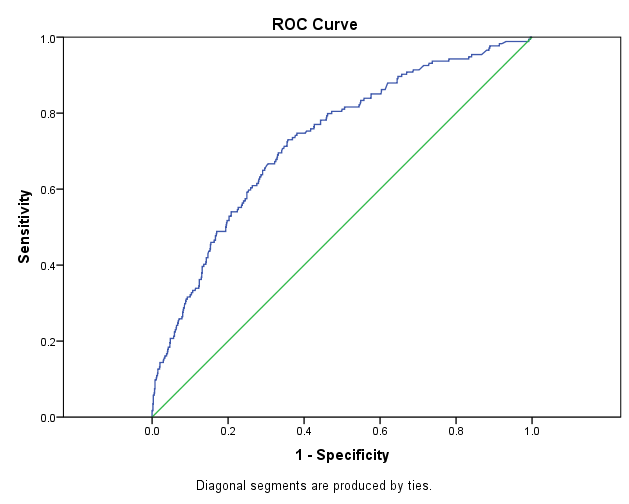
\includegraphics[height=1.2in]{ML_ROC.png}
%\caption{\fontsize{7.2pt}{4.2pt}\selectfont{评估机器学习模型的混同矩阵和\textrm{ROC}示意,理想的混同矩阵是单元阵,\textrm{ROC}以下的面积越大,表示模型的性能越好.}}%
\label{ML_CM_ROC}
\end{figure}
不同阈值下的\textrm{ROC}曲线反应了模型的预测能力}}
}

\frame
{
	\frametitle{机器学习的验证}
{\fontsize{7.0pt}{4.2pt}\selectfont{回归预测也有很多方案可以评估模型对数据的拟合精度,如:
\begin{itemize}
	\item 平均绝对误差\textrm{(mean absolute error, MAE)}
		\begin{displaymath}
			\mathrm{MAE}=\dfrac1n\sum_i^n|y_i-\hat{y}_i|
		\end{displaymath}
	\item 归一化相对百分误差\textrm{(normalized mean absolute in percentage, MAPE)}
		\begin{displaymath}
			\mathrm{MAPE}=\dfrac{100\%}n\sum_i^n\dfrac{y_i-\hat{y}_i}{y_i}
		\end{displaymath}
	\item 均方误差\textrm{(mean squared error, MSE)}
		\begin{displaymath}
			\mathrm{MSE}=\dfrac1n\sum_i^n(y_i-\hat{y}_i)^2
		\end{displaymath} 
{\fontsize{5.0pt}{4.2pt}\selectfont{从使用频率角度说,由分布参数$\theta$估计$\hat{\theta}^m$与\textrm{MSE}密切关联,即
		\begin{displaymath}
			\mathrm{MSE}=\mathtt{E}[(\hat{\theta}_m-\theta)^2]=\mathrm{Bias}(\hat{\theta}_m)^2-\mathrm{Var}(\theta)
		\end{displaymath}
		一般更常用的是误差的均方根\textrm{(root of MSE, RMSE)}}}
\end{itemize}
\vskip 2pt
		还有用可决统计系数(也称决定系数,\textrm{coefficient of determination})~$\mathrm{R}^2$
		\vskip 2pt
		{\fontsize{6.0pt}{4.2pt}\selectfont{可决统计系数的定义为$\mathrm{R}^2=1-\frac{\mathrm{SS}_{\mathrm{res}}}{\mathrm{SS}_{\mathrm{tot}}}$}}\\
		{\fontsize{5.0pt}{4.2pt}\selectfont{这里$\mathrm{SS}_{\mathrm{res}}=\sum\limits_i(y_i-\bar{y})^2$是总的方差求和,而$\mathrm{SS}_{\mathrm{res}}=\sum\limits_i(y_i-\hat{y}_i)^2$是预测模型误差平方求和}}
	}} }

\section{数据挖掘与第一原理材料研究}
\frame
{
	\frametitle{材料信息学\textrm{(Materials Informatics)}与数据挖掘}
%信息科学与生物学的交叉形成生物信息学极大地带动了信息学科与基础学科的融合
	材料信息学:~{\fontsize{8.0pt}{4.2pt}\selectfont{\textcolor{blue}{应用数据挖掘特别是机器学习技术推动材料科学研究}
	\begin{itemize}
		\item 材料信息学主要研究材料的内禀特征\textrm{(intrinsic features)},包括结构、组成、对称性等与材料的性质间的内在数据关联
		\item 材料学研究的数据挖掘主要是监督学习,即材料物性的预测和材料的分类
			\begin{itemize}
{\fontsize{7.0pt}{4.2pt}\selectfont{
\item \textcolor{magenta}{物性预测}:~应用包括回归在内的学习算法,建立材料物性的描述函数$f(\mathbf{x})$
\item \textcolor{magenta}{分类问题}:~根据特定的物性目标,将符合要求的材料归入其中}}\\%
					{\fontsize{5.0pt}{4.2pt}\selectfont{比如按磁性和非磁性划分,按照晶体所属结构分类属于两种不同分类,每种分类方式内部各部分之间不存在交集}}
	\end{itemize}
	\end{itemize}
%。通常材料科学研究的习惯思路是已知材料的特征$x_i$,则其影响的材料性质$y_i=f(x_i)$将会如何变化,确定\{\textit{材料}$\rightarrow$\textit{性质}\}的映射关系;~而对于新材料开发领域,往往有逆向式思维,为了获得具有某种性质的材料,则必须使其存在哪些内禀特征。事实上,只有以数据驱动的材料学研究模式,才是能同时回答上述问题的主要形式。

%材料科学中数据挖掘特别是机器学习研究的一般思路
\begin{figure}[h!]
\centering
%\vspace*{-0.1in}
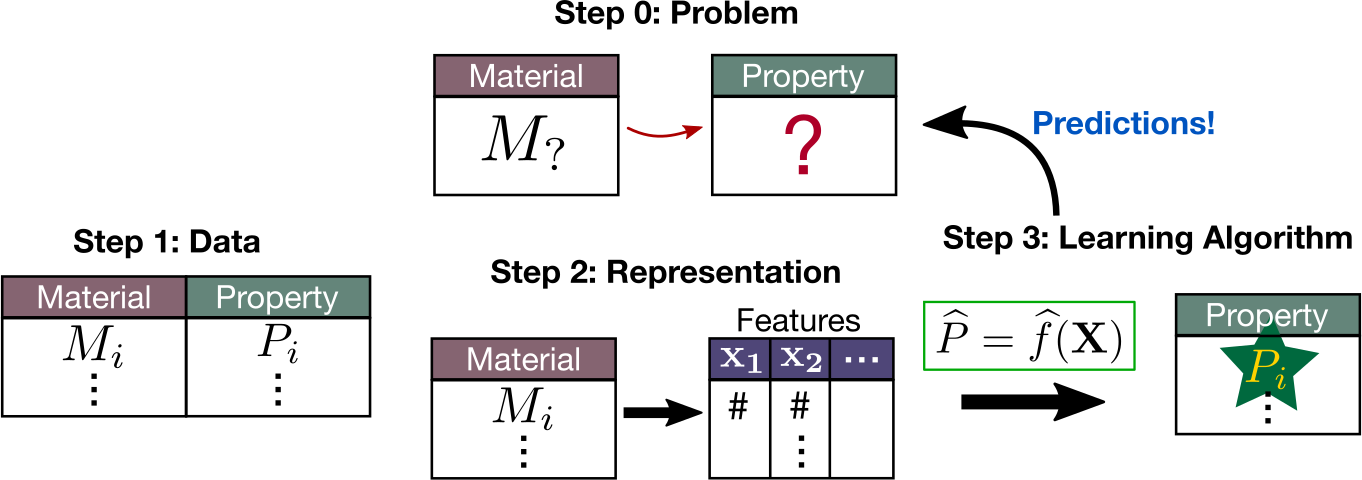
\includegraphics[height=1.4in]{Materials_informations_workflow.png}
\caption{\tiny{\textrm{General Process of Data Mining in Materials Science}}}%.引自文献\inlinecite{NPJCM3-54_2017}}}}%
\label{npjCM}
\end{figure}}}
}

\frame
{
	\frametitle{数据驱动的材料研究主要流程}
在数据挖掘驱动的材料计算的主要研究流程为:
\begin{enumerate}
	\item \textcolor{purple}{问题的确定}:~根据问题类型选择机器学习算法\\
%		{\fontsize{6.0pt}{4.2pt}\selectfont{\textcolor{blue}{机器学习特征向量的确定:~平衡算法与效率}}}
	\item \textcolor{purple}{数据的组织}:~数据应该涵盖研究样本的全部特征(输入)和目标物性(输出)\\
		{\fontsize{6.0pt}{4.2pt}\selectfont{\textcolor{blue}{数据是机器学习的基本对象,可以来自理论计算,也可来自实验测量}}}
	\item \textcolor{purple}{物性的表示}:~描述符决定机器学习的性能\\
		{\fontsize{6.0pt}{4.2pt}\selectfont{\textcolor{blue}{描述材料物性的特征向量称为描述符}}}
	\item \textcolor{purple}{算法和模型的选定、评估与优化}:~主要针对超参数的选择\\
		\begin{itemize}
			\item {\fontsize{6.0pt}{4.2pt}\selectfont{考虑模型的复杂度/合理性}}
			\item {\fontsize{6.0pt}{4.2pt}\selectfont{算法的精度-效率/性能和训练时长平衡}}
		\item {\fontsize{6.0pt}{4.2pt}\selectfont{既要防止数据不足也要防止过拟合}}
		\end{itemize}
\end{enumerate}
机器学习的建模可以简单概述为
\begin{displaymath}
	\mbox{\textcolor{red}{机器学习模型}=\textcolor{magenta}{研究对象}+\textcolor{magenta}{数据}+\textcolor{magenta}{表示}+\textcolor{magenta}{学习算法}+\textcolor{magenta}{优化}}
\end{displaymath}
}

\frame
{
	\frametitle{机器学习预测材料性质}
\begin{figure}[h!]
\centering
\vspace*{-0.1in}
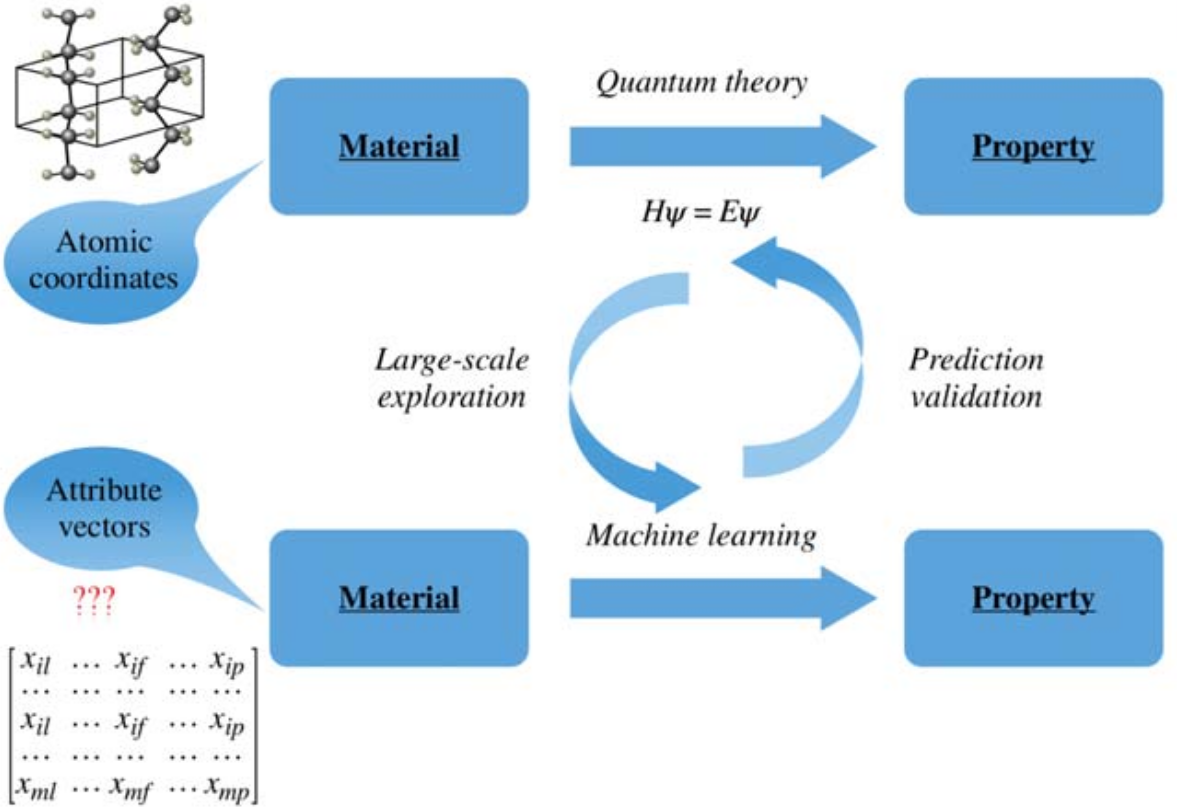
\includegraphics[height=2.5in]{ML_DFT-1.png}
\caption{\tiny{\textrm{Making machine-learning prediction replacing the expensive quantum chemistry calculation.}}}%
\label{ML_QM}
\end{figure}
}

\frame
{
	\frametitle{机器学习对\textrm{DFT}的促进}
机器学习在第一原理计算领域重要的作用:~节省或替代获取\textrm{DFT}计算结果或数据所必需的成本
\begin{itemize}
	\item 对复杂电子体系,\textrm{Schr\"odinger}方程直接的迭代求解对计算资源和时间成本都比较高
	\item \textrm{DFT}框架下,机器学习加速\textrm{Kohn-Sham}方程求解:~避免直接求解\textrm{Kohn-Sham}方程,直接预测电子密度\\
		{\fontsize{8.0pt}{4.2pt}\selectfont{通过机器学习获得材料的电子密度-势的映射关系,得到能量泛函后,对能量泛函求变分极小得到基态能量}}
	\item 优化\textrm{DFT}计算的能量泛函,可将机器学习方法很方便地与传统\textrm{DFT}计算结合起来使用\\
		{\fontsize{8.0pt}{4.2pt}\selectfont{机器学习优化的泛函并不限于传统\textrm{DFT}的\textrm{Kohn-Sham}方程的交换-相关部分,也可以用于无轨道类型\textrm{(free-orbital)}的能量密度泛函}}
\end{itemize}
{\fontsize{7.0pt}{4.2pt}\selectfont{
\begin{itemize}
	\item 机器学习还可用于解决量子多体问题:~得到紧束缚模型的类\textrm{Schr\"odinger}方程的\textrm{Hamiltonian}
	\item 机器学习应用于计算材料研究,特别是在大于电子尺度的材料计算,还包括计算配分函数、寻找相变和序参量以及获得模型的\textrm{Green's function}等
\end{itemize}}}
}

\frame
{
	\frametitle{机器学习对\textrm{DFT}的促进}
\begin{figure}[h!]
\centering
\vspace*{-0.1in}
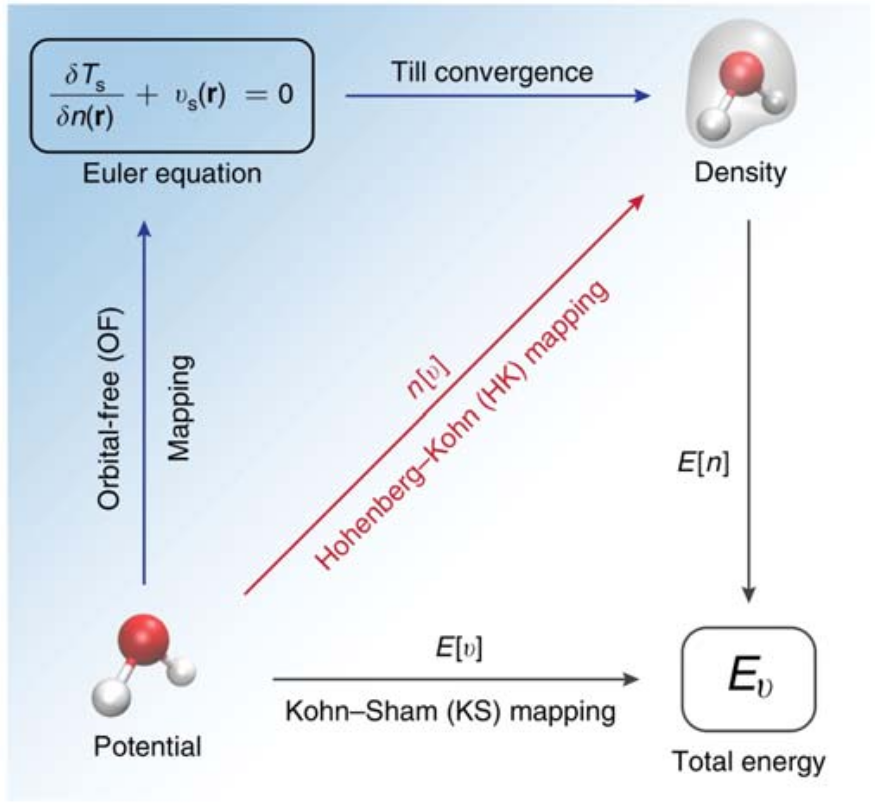
\includegraphics[height=2.3in]{ML_DFT-2.png}
%\caption{\tiny{\textrm{Three main ways of machine-learning supporting DFT calculation.}}}%
\label{ML_DFT}
\end{figure}
	{\fontsize{8.0pt}{4.2pt}\selectfont{机器学习这些领域的成功应用:~\textcolor{red}{展示了数据挖掘技术在拓展材料科学研究前沿有着广阔的应用前景,可应用于多种尺度下材料学研究的各类系统和现象}}}
}

%\subsection{机器学习在第一原理材料研究中的应用}
%\frame
%{
%\frametitle{新材料发现及稳定性}
%机器学习用于材料学研究的主要目标是通过数据驱动加速新的物质(主要是各类化合物)的发现。具体地说,通过机器学习,可以阐述材料的热力学稳定性,从而有效地预测化合物的形成能。\textrm{Curtarolo}和\textrm{Ceder}等是利用诸如\textrm{PCA}、线性回归等机器学习方法来预测晶体结构、形成能并优化高通量计算的先驱,、\textrm{Hautier}等应用机器学习方法,由\textrm{ICSD}的实验数据确定新的三元化合物的主要元素组成,并用高通量计算模拟验证。\textrm{Saad}等用二元化合物为样本,介绍了机器学习的基本概念和监督学习与无监督学习降维技术。\textrm{Patra}等应用偏倚神经网络遗传算法\textrm{(neural-newwork-biased genetic algorithm, NBGA)}加速特定物性材料的设计,通过人工神经网络遗传算法的筛选优化,对模拟或实验样本数据按照类似生物进化的多代筛选,获得特定物性的提升。采用随机森林算法,预测\textrm{Heusler}合金时,仅以元素组分为特征向量(描述符),得到很理想的结果,并且很快得到实验合成的验证。\textrm{Faber}等对\textrm{ICSD}数据库中大量化合物的形成能应用\textrm{kernel ridge}回归,发现平均误差在0.1\textrm{eV/atom}的钾冰晶石化合物(\ch{ABC2D6})结构约90种。

%\textrm{Okamoto}在材料科学的化学组分研究中,应用\textrm{Bayesian}方法,只在6\%的搜索空间中就找到了嵌入金属锂的石墨烯稳定化学物\cite{JPCA121-3299_2017}。

%预测晶体结构及其稳定性
%}

%------------------------------------------------------------------------Reference----------------------------------------------------------------------------------------------
		\frame[allowframebreaks]
{
\begin{thebibliography}{99}
\frametitle{主要参考文献}
{\tiny
\bibitem{NPJCM3-54_2017}\textrm{R. Ramprasad and R. Batra and G. Pilania and A. Mannodi-Kanakkithodi and C. Kim. \textit{npj. Comput. Mater.}, \textbf{3} (2017), 54}
\bibitem{NNature559-547_2018}\textrm{K. T. Butler and D. W. Davies and H. Cartwright and O. Isayev and A. Walsh. \textit{Nature}, \textbf{559} (2018), 547}
\bibitem{COSSMS21-167_2016}\textrm{L. Ward and C. Wolverton \textit{Curr. Opin. Solid State Mater. Sci.}, \textbf{21} (2016), 167}
\bibitem{JM3-519_2017}\textrm{Y. Liu and T. Zhao and W. Ju and S. Shi \textit{J. Materiomics.}, \textbf{3} (2017), 519}
}
\end{thebibliography}
%\nocite*{}
}

\appendix
%\frame
%{
%	\frametitle{卖油翁}
%%陈康肃公尧咨善射,当世无双 ,公亦以此自矜。尝射于家圃,有卖油翁释担而立,睨之,久而不去。见其发矢十中八、九,但微颔之。康肃问曰:“汝亦知射乎?吾射不亦精乎?”翁曰:“无他,但手熟尔。”康肃忿然曰:“尔安敢轻吾射!”翁曰:“以我酌油知之。”乃取一葫芦置于地,以钱覆其口,徐以杓酌油沥之,自钱孔入而\footnote{一作“而入”}钱不湿。因曰:“\textcolor{red}{我亦无他,惟手熟尔}。”康肃笑而遣之。此与庄生所谓“解牛”、“斫轮”者何异?
%\begin{figure}[h!]
%\centering
%\vspace{-10.5pt}
%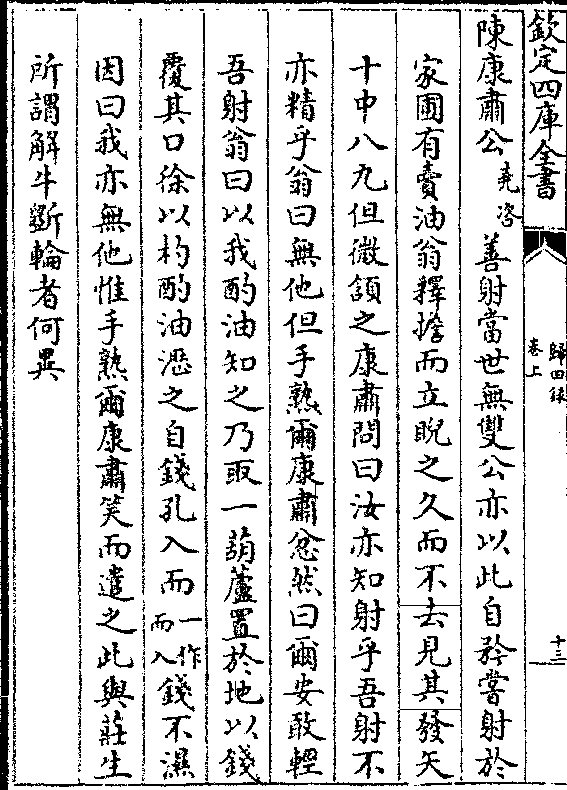
\includegraphics[height=0.65\textwidth]{Figures/Sale_Oil_Ouyang.png}
%\hspace{1pt}
%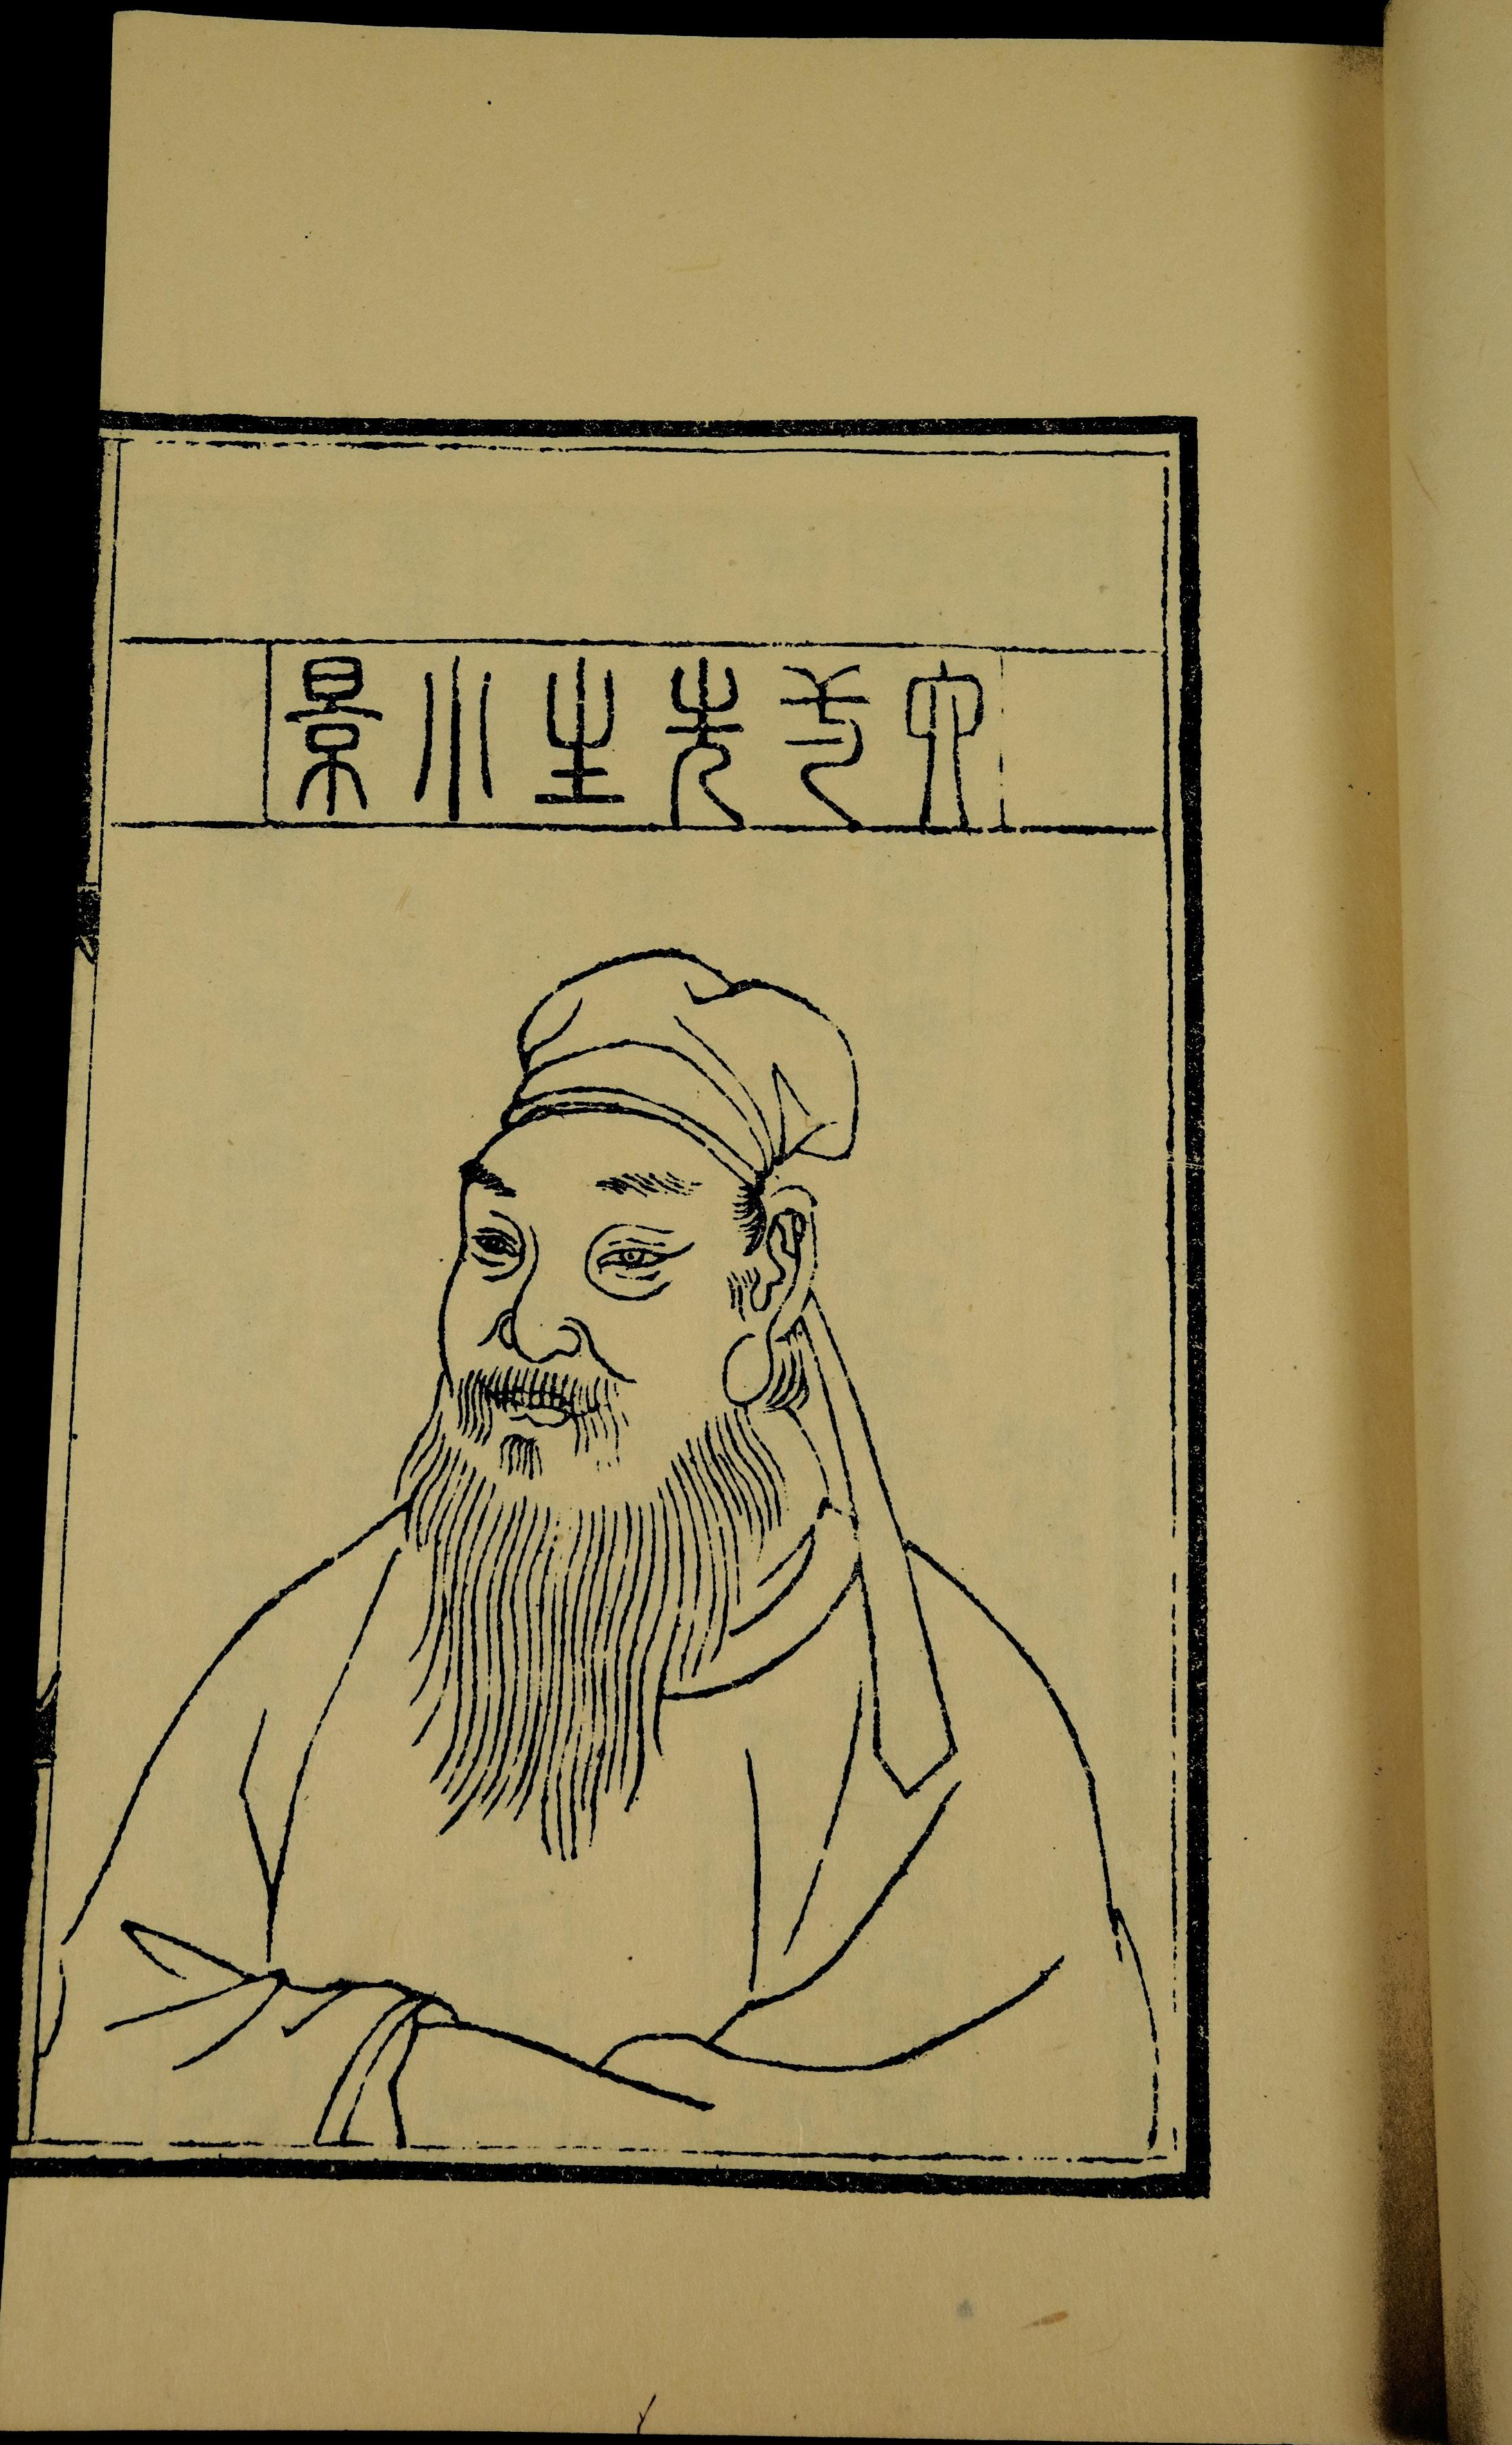
\includegraphics[height=0.65\textwidth]{Figures/Ouyang_Xiu-2.jpg}
%\caption{\fontsize{6.2pt}{5.2pt}\selectfont{欧阳修\textrm{(1007-1072)}~《欧阳文忠公文集$\cdot$归田录》~卷上}}
%\label{Sale_oil}
%\end{figure}
%}

%\frame
%{
%	\frametitle{向我国固体物理学科的奠基人致敬!}
%\begin{figure}[h!]
%\centering
%\vspace{-15.5pt}
%\subfigure[\fontsize{6.3pt}{5.2pt}\selectfont{黄~~昆教授\textrm{(1919-2005)}}]{
%\label{fig:Huang}
%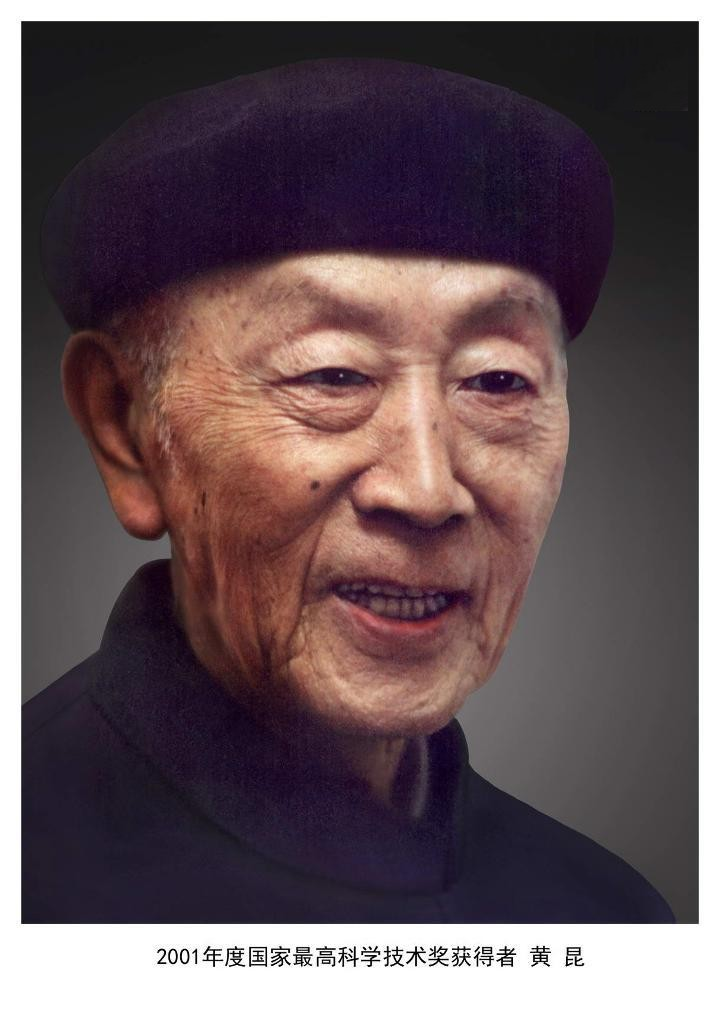
\includegraphics[height=1.20in,width=1.9in,viewport=-300 90 1020 1000,clip]{Figures/Huang.jpg}}
%\subfigure[\fontsize{6.3pt}{5.2pt}\selectfont{谢希德教授\textrm{(1921-2000)}}]{
%\label{fig:Xie}
%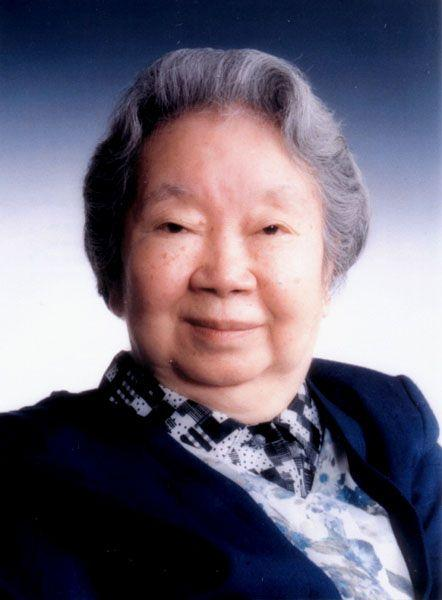
\includegraphics[height=1.20in,width=1.9in,viewport=-210 0 630 575,clip]{Figures/Xie.jpg}}
%\subfigure[\fontsize{6.3pt}{5.2pt}\selectfont{彭桓武研究员\textrm{(1915-2007)}}]{
%\label{fig:Peng}
%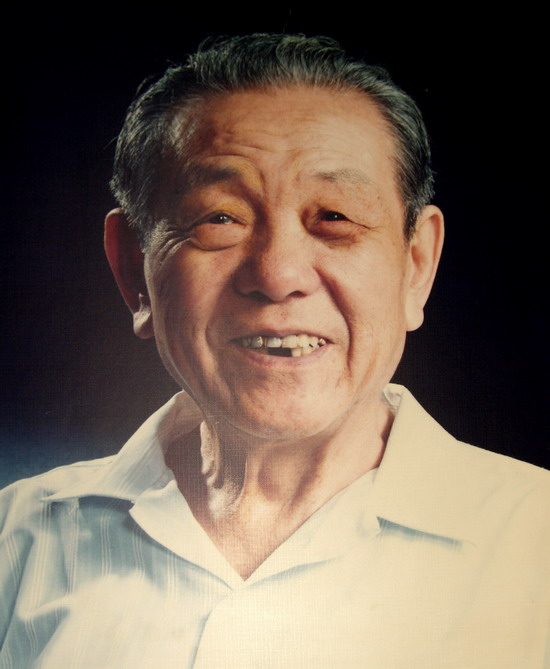
\includegraphics[height=1.20in,width=1.9in,viewport=-270 0 810 660,clip]{Figures/Peng.jpg}}
%\subfigure[\fontsize{6.3pt}{5.2pt}\selectfont{程开甲教授\textrm{(1918-2018)}}]{
%\label{fig:Cheng}
%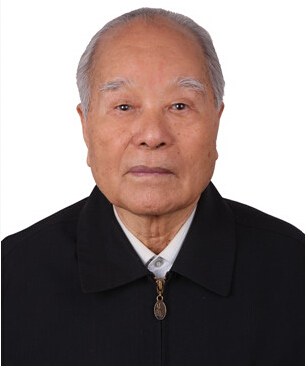
\includegraphics[height=1.20in,width=1.9in,viewport=-110 0 325 275,clip]{Figures/Cheng.jpg}}
%%\caption{}%
%\label{Peng_Huang_Xie_Cheng}
%\end{figure}
%}
%
%\frame
%{
%	\frametitle{向我国量子化学学科的奠基人致敬!}
%\begin{figure}[h!]
%	\centering
%\centering
%\vspace{-10.5pt}
%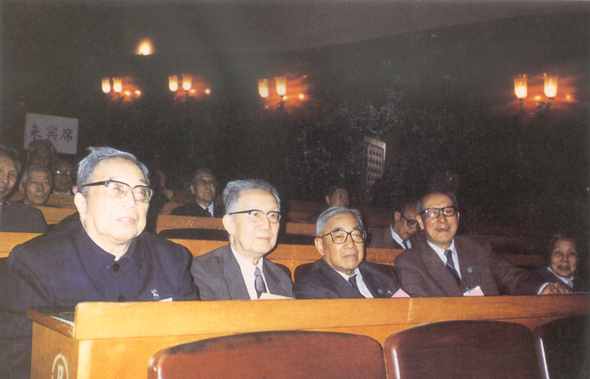
\includegraphics[height=0.58\textwidth,width=1.01\textwidth,viewport=0 0 435 250,clip]{Figures/1994_6_5.jpg}
%\caption{\fontsize{6.3pt}{5.2pt}\selectfont{\textrm{1994}年\textrm{6}月\textrm{5}日,唐敖庆教授\textrm{(1915-2008)}、吴征铠教授\textrm{(1913-2007)}、卢嘉锡教授\textrm{(1915-2001)}、徐光宪教授\textrm{(1920-2015)}和高小霞教授\textrm{(1919-1998)}(从左到右)在第七次院士大会上}}
%%\caption{1994年6月5日\fbox{唐敖庆}教授、\fbox{吴征铠}教授、\fbox{卢嘉锡}教授、\fbox{徐光宪}教授和\fbox{高小霞}教授(从左到右)在第七次院士大会上}
%%\caption{1994年6月5日\frame{唐敖庆}教授、\frame{吴征铠}教授、\frame{卢嘉锡}教授、\frame{徐光宪}教授和\frame{高小霞}教授(从左到右)在第七次院士大会上}
%\label{Tang_Wu_Lu_Xu}
%\end{figure}
%}

\frame
{
	\frametitle{}
\begin{figure}[h!]
\centering
\vspace{-5.5pt}
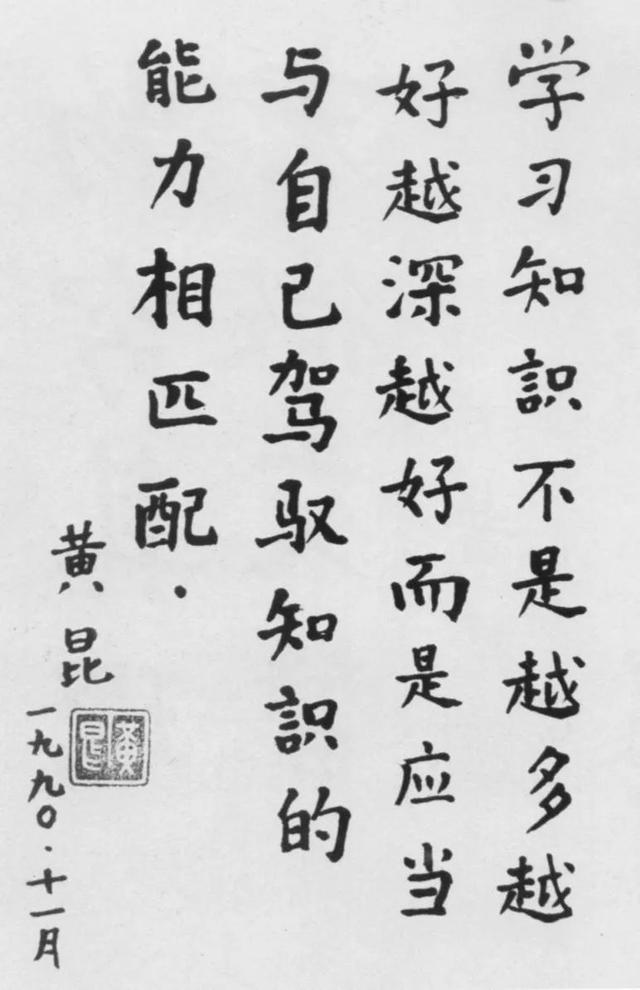
\includegraphics[height=0.65\textwidth]{Figures/Quote-Huang_Kun.jpg}
\caption{\fontsize{6.2pt}{5.2pt}\selectfont{黄~~昆~教授的治学箴言}}
\label{Quote-Huang_Kun}
\end{figure}
}

\frame
{
\begin{figure}[h!]
\vskip -5pt
\centering
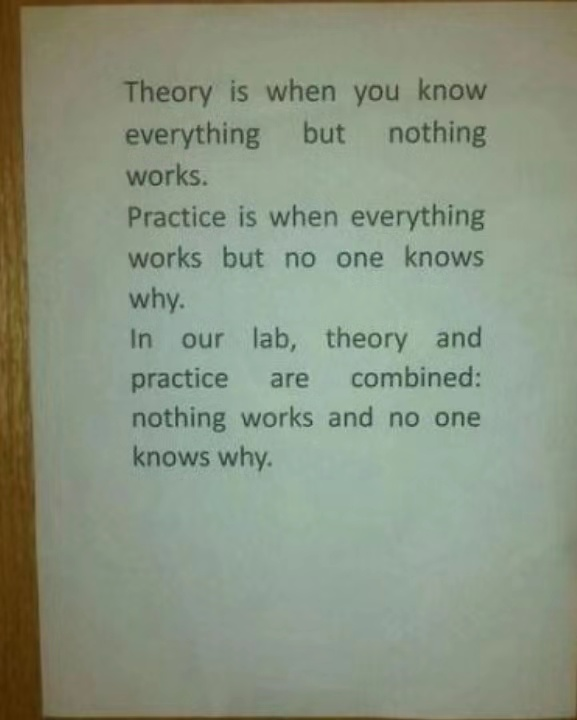
\includegraphics[height=2.8in,width=2.3in,viewport=30 65 444 600,clip]{Figures/Theory_Practice.jpg}
\label{Theory_Practice}
\end{figure}
}

